\documentclass[12pt,a4paper, oneside]{book}
\usepackage{fancyhdr, amsmath}
\usepackage{epsfig, graphics, graphicx,subfigure}
\graphicspath{/figuras}
%\psdraft
\pagestyle{fancy}
\renewcommand{\chaptermark}[1]{\markboth{\thechapter.#1}{}}
\renewcommand{\sectionmark}[1]{\markright{\thesection.#1}}
\fancyhead[le,ro]{\textbf{\thepage}}
\fancyhead[re]{\textbf{\leftmark}}
%\fancyhead[lo]{\textbf{\rightmark}}
%\fancyfoot[le,lo]{\textbf{Estudio te\'orico y experimental de propiedades magn\'eticas en materiales bidimensionales}}
%\fancyfoot[ro]{\textbf{}}
%\fancyfoot[ro]{}
\renewcommand{\headrulewidth}{0.15mm}
\renewcommand{\footrulewidth}{0.15mm}
\addtolength{\headwidth}{\marginparsep}
\addtolength{\headwidth}{\marginparwidth}
\usepackage[spanish]{babel}

\begin{document}
	\tableofcontents
	\listoffigures
	\chapter{Introducci\'on}
	en el presente trabajo se muestra un estudio  te\'orico de materiales bidimensionales para poder encontrar su respuesta 
	\chapter{Teor\'ia funcional de la densidad} \label{cap:DFT}
	En este cap\'itulo se describe la teor\'ia que se necesita para realizar las simulaciones de los materiales realizadas en este trabajo, comenzando con explicar de forma general en que consiste la teoría funcional de la densidad para posteriormente mostrar la teor\'ia realizada por Kohn-Sham y explicar las ecuaciones que se surgen de este an\'alisis adem\'as que se explica el m\'etodo de soluci\'on y la manera en que se  emplean para calcular las distintas propiedades de materiales.
	\newline 
	\section{Introducci\'on a la teor\'ia funcional de la densidad} \label{sec:introdft}
	
	La ecuaci\'on fundamental para la descripci\'on de todas las propiedades de los materiales es la ecuaci\'on  de  sch\"odringer para muchos cuerpos: en donde el Hamiltoniano est\'a dada por:
	\begin{multline}
	\hat H = - \frac{\hbar ^2}{2 m_e} \sum_{i} \nabla_{i}^2 - \sum_{i,I} \frac{Z_I e^2}{\vert \pmb{r_i} - \pmb{R_I} \vert}+ \frac{1}{2} \sum_{i \not= j}  \frac{e^2}{|\pmb{r_i} - \pmb{r_j} |}\\
	- \sum_{I} \frac{\hbar^2}{2 M_I} \nabla_I^2 + \frac{1}{2} \sum_{I \not= J} \frac{Z_I Z_J e^2}{|\pmb{R_I}-\pmb{R_J}|}  \label{ec:sh} 
	\end{multline}	
	\newline
	en donde las posiciones de los electrones se escriben en letras min\'usculas y los n\'ucleos con n\'umero at\'omico  $Z_I$, en la posici\'on $\pmb{R_I}$ y masa $M_I$ se representan con letras may\'usculas,el problema a resolver es encontrar m\'etodos para tratar con  los efectos de las interacci\'on  electr\'on-electr\'on que son fundamentales para describir los fenómenos en los materiales, si se observa la ecuaci\'on \ref{ec:sh} se nota que no es posible resolver la ecuaci\'on de sch\"odringer ni de forma anal\'itica ni num\'erica debido a que se tiene que resolver para una gran n\'umero de part\'iculas por lo tanto se tienen que realizar aproximaciones para poder tratar con este problema.
	\newline
	Debido a que nos interesa principalmente las interacciones electr\'on-electr\'on lo primero que se podr\'ia intentar hacer es desacoplar las variables de los n\'ucleos  y de los electrones, esto no es posible debido a que en la ecuaci\'on \ref{ec:sh} se tienen las interacciones electr\'on-n\'ucleo, para poder desacoplar estas variables se utiliza la aproximaci\'on de Born-Oppenheimer, tambi\'en llamada aproximaci\'on adiabática, consiste en observar que los protones y neutrones en el n\'ucleo son mucho mas masivos que los electrones por lo tanto el movimiento de los n\'ucleos es mucho mas pequeño que el  los electrones, entonces por consecuencia, los electrones pueden  responder la movimiento de los n\'ucleos casi instant\'aneamente, por otro lado tambi\'en se puede decir que los n\'ucleos no pueden seguir el movimiento de los electrones por lo tanto se puede omitir el cuarto t\'ermino en la ecuaci\'on \ref{ec:sh} el cual corresponde a la energ\'ia cin\'etica de los n\'ucleos, por este motivo se asume que la posiciones $\pmb{R_I}$ est\'an fijas y el \'ultimo t\'ermino de ña ecuaci\'on \ref{ec:sh} es una constante que recorre la energ\'ia total de los electrones.
	\newline
	Tomando todo esto en consideraci\'on la ecuaci\'on \ref{ec:sh} se puede escribir como:
	 \begin{equation}
	 \hat H = \hat T + \hat V_{ext} + \hat V_{int}+E_{II} \label{ec:shelectron}
	 \end{equation}
	cuyos t\'erminos expresados en unidades at\'omicas de Hartree ($\hbar = m_{e} = e= 4\pi / \epsilon_0 =1 $)  corresponden al operador de energ\'ia cin\'etica de los electrones $\hat T$
	\begin{equation}
	\hat{T} = \sum_{i} -\frac{1}{2} \nabla_{i}^2 \label{ec:shT}
	\end{equation}
	$\hat{V}_{ext}$ es el potencial entre electrones y n\'ucleos
	\begin{equation}
	\hat{V}_{ext} = \sum_{i,I} V_I (|\pmb{r_i}-\pmb{R_I}|) \label{ec:shVex}
	\end{equation}
	$\hat{V}_{int}$ es el potencial de la interacci\'on electr\'on-electr\'on
	\begin{equation}
	\hat{V}_{int} = \frac{1}{2} \sum_{i \not= j} \frac{1}{|\pmb{r_i}-\pmb{r_j}|} \label{ec:shVint}
	\end{equation}
	y el \'ultimo  t\'ermino $E_{II}$ corresponde a la constante descrita anteriormente que muestra la interacci\'on entre los n\'ucleos. La ecuaci\'on \ref{ec:shVex} es llamado tambi\'en potencial externo con respecto a los electrones, este potencial generalmente se asume que es una interacci\'on Coulombica aunque puede ser remplazado por un pseudopontencial que tome en cuenta los efectos de los electrones mas cercanos al n\'ucleo, tambi\'en se  pueden agregar otros "potenciales externos" tales como campos el\'ectricos o de t\'erminos Zeeman para campos magn\'eticos. 
	\newline
	\newline
	La ecuaci\'on fundamental que gobierna un sistema cu\'antico es la ecuaci\'on de Sch\"odringer
	\begin{equation}
	i \hbar \frac{d \Psi ({\pmb{r}_i}; t)}{dt} = \hat H \Psi ({\pmb{r}_i}; t) \label{ec:shtime}
	\end{equation}
	en donde $\Psi ({\pmb{r}_i}; t) \equiv \Psi ({\pmb{r}_1, \pmb{r}_2, ... ,\pmb{r}_n }; t) $ es la funci\'on de onda de muchos cuerpos y es spin se asume que est\'a incluido en la posici\'on $\pmb{r}_i$ adem\'as que la funci\'on de onda es antisim\'etrica al intercambio de las posiciones. Observando que el Hamitoniano (ec.\ref{ec:sh}) no depende del tiempo entonces los eigenvalores de la ecuaci\'on \ref{ec:shtime} se pueden escribir como $ \Psi ({\pmb{r}_i}; t) =  \Psi ({\pmb{r}_i}) e^{(i E/ \hbar) t} $, el siguiente paso es tratar de aproximar este problema de muchos cuerpos a uno, por lo que la  ecuaci\'on de sch\"odringer independiente del tiempo tendr\'ia la siguiente forma:
	\begin{equation}
	\hat H _{eff} \Psi_{i,s} (\pmb{r}) = \left [ -\frac{\hbar^2}{2m_e} \nabla^2 + V_{eff}^{s} \right]\Psi_{i,s} (\pmb{r}) = \varepsilon_i ^{s} \Psi_{i,s} (\pmb{r})  \label{ec:shuncuerpo}
	\end{equation}
	en donde $V_{eff}^{s}$ es el potencial que siente un electr\'on de spin $s$ y posici\'on $\pmb{r}$, en el estado base los electrones ocupan los eigenvalores menores obedeciendo el principio de exclusi\'on. Conociendo que los eigenestados de la ecuaci\'on \ref{ec:shuncuerpo} son ortogonales, se puede formar una funci\'on de onda antisim\'etrica con el determinante de estos eigenestados el cual se le llama determinante de Slater, el cual tiene la siguiente forma:
	\begin{equation}
	\Psi = \frac{1}{\sqrt{N !}}
	\begin{vmatrix}
	\phi_1 (\pmb{r}_1, s_1) & \phi_1 (\pmb{r}_2, s_2) & \phi_1 (\pmb{r}_3, s_3) & \cdots & \phi_1 (\pmb{r}_N, s_N) \\
	\phi_2 (\pmb{r}_1, s_1) & \phi_2 (\pmb{r}_2, s_2) & \phi_2 (\pmb{r}_3, s_3) & \cdots & \phi_2 (\pmb{r}_N, s_N)\\
	\phi_3 (\pmb{r}_1, s_1) & \phi_3 (\pmb{r}_2, s_2) & \phi_3 (\pmb{r}_3, s_3) & \cdots & \phi_3 (\pmb{r}_N, s_N) \\
	                       &  \vdots                     & \vdots                      &  \ddots & \vdots\\
	\phi_N (\pmb{r}_1, s_1) & \phi_N (\pmb{r}_2, s_2) & \phi_N (\pmb{r}_3, s_3) & \cdots & \phi_N (\pmb{r}_N, s_N) \\
	  
	\end{vmatrix} \label{ec:slater}
	\end{equation}
	en donde $\phi_i (\pmb{r}_i s_i)$ es la funci\'on de onda de un solo orbital y N es el n\'umero de electrones en el sistema.
	\newline
	Utilizando esta aproximaci\'on es posible definir expresiones que son necesarias para la teor\'ia funcional de la densidad,se puede definir el valor promedio cualquier operador de la siguiente manera:
	\begin{equation}
	\langle \hat{O} \rangle= \sum_{i} f_{i,s} \langle \Psi_{i,s} | \hat{O} | \Psi_{i,s}\rangle \label{ec:prom}
	\end{equation} 
	\newline
	en donde $\langle \Psi_{i,s} | \hat{O} | \Psi_{i,s} \rangle$ es el valor de espectaci\'on del operador $\hat{O}$ y $f_{i}^{s}$ es la distribuci\'on de Fermi-Dirac, definida por:
	\begin{equation}
	f_{i}^{s}= \frac{1}{e^{\beta (\varepsilon_{i,s}-\mu)}+1} \label{ec:fermi-dirac}
	\end{equation}
	en donde $\beta= \frac{1}{k_B T}$, $\mu$ es la energ\'ia de Fermi y $\varepsilon_{i,s}$ es la energ\'ia de una part\'icula sin interacci\'on dada por $\langle \Psi_{i,s} | \hat{H} | \Psi_{i,s}\rangle$, entonces el valor promedio de la energ\'ia est\'a dado por:
	\begin{equation}
	\langle E \rangle = \langle \hat{H} \rangle = \sum_{i} f_{i,s} \langle \Psi_{i,s} | \hat{H} | \Psi_{i,s}\rangle = \sum_{i} f_{i,s}  \varepsilon_{i,s} \label{ec:energia1}
	\end{equation}
	la siguiente simplificaci\'on que se realiza es que la distribuci\'on de Fermi-Dirac a temperatura de cero grados Kelvin se puede aproximar como 1 para los estados por de bajo del nivel de Fermi y 0 para los dem\'as, utilizando esto se puede escribir la ecuaci\'on \ref{ec:energia1} como
	\begin{equation}
	E= \langle \Psi | \hat{H} | \Psi \rangle \label{ec:energia}
	\end{equation}
	en donde $\Psi$ es el determinarte de Slater (ec. \ref{ec:slater})
	\newline
	Otra cantidad de gran importancia es la densidad, para la cual se puede definir como:
	\begin{equation}
	\hat{\rho}_{s ', s}= \sum_{i} | \psi_{i,s '} \rangle n_{i,s} \langle \psi_{i,s} | \label{ec:densidad}
	\end{equation}
	en donde $ n_{i,s} $ es el n\'umero de ocupaci\'on para el nivel $i$ y spin $s$ y toma valores de 1 y 0 por los motivos antes mencionados, de hay que recordar que es posible reescribir la ecuaci\'on \ref{ec:prom} como $\langle \hat{O} \rangle = Tr \hat{\rho} \hat{O}  $, se puede obtener una expresi\'on para la densidad:
	\begin{equation}
	n_{s ', s} (\pmb{r ', r} ) = \delta_{s',s} \sum_{i} \psi_{i,s} ^{ *} (\pmb{r'}) n_{i,s} \psi_{i,s } (\pmb{r})  \label{ec:densidadr}
	\end{equation}
	si se tiene que $\pmb{r'} = \pmb{r}  $ y $s = s '  $ se tiene una erxpresi\'on para la densidad electr\'onica con spin $s$:
	\begin{equation}
	n(\pmb{r})= \sum_{i} n_{i,s} | \psi_{i,s} (\pmb{r}) |^2 \label{ec:densTot}
	\end{equation}
	o en el caso de que $s \not = s '  $:
	\begin{equation}
	n_{s ', s }(\pmb{r})= \delta_{s',s} \sum_{i} \psi_{i,s '}^ {*} (\pmb{r}) n_{i,s}~ \psi_{i,s } (\pmb{r}) \label{ec:denspin}
	\end{equation}
	as\'i mismo es posible definir la densidad de magnetizaci\'on utilizando la ecuaci\'on \ref{ec:denspin} y tomando en cuenta que $s, s ' = \uparrow, \downarrow $ adem\'as de considerar solo la contribuci\'on del spin del electr\'on:
	\begin{equation}
	\pmb{m} (\pmb{r}) = - \mu_{B} \sum_{s,s '} \pmb{\sigma}_{s,s'} n_{s ', s }(\pmb{r}) \label{ec:magn}
	\end{equation}
	en donde $\mu_B= \frac{e \hbar}{2 m} = 0.579 \times 10^{-4} \frac{eV}{T}$ es el magnet\'on de Borh y $ \pmb{\sigma}_{s,s'}$ es el vector formado por las matrices de Pauli, sabiendo esto es posible escribir las componentes de la ecuaci\'on \ref{ec:magn}:
	\begin{subequations} \label{ec:compm}
		\begin{gather}
		m_x (\pmb{r})= -2 \mu_{B} Re~ n_{\uparrow, \downarrow} (\pmb{r}) \label{ec:compm1}\\
		m_y (\pmb{r})= -2 \mu_{B} Im~ n_{\uparrow, \downarrow} (\pmb{r}) \label{ec:compm2}\\
		m_z (\pmb{r}) = - \mu_{B} [n_{\uparrow, \uparrow} (\pmb{r})- n_{\downarrow, \downarrow} (\pmb{r})] \label{ec:compm3}
		\end{gather}
	\end{subequations}
  
  Si la densidad de magnetizaci\'on est\'a dirigida solamente en la direcci\'on z, entonces se dice que es colineal, en caso contrario es no colineal. 
  \newline \newline
  Tras haber hecho estas definiciones es ahora el turno de definir la energ\'ia descrita por la ecuaci\'on \ref{ec:energia} utilizando el Hamiltoniano de la ecuaci\'on \ref{ec:shelectron}, adem\'as se considera el caso colineal y sin el acople de spin-\'orbita, tomando esto en consideraci\'on las funciones de los orbitales de la ecuaci\'on \ref{ec:slater} se pueden representar como el producto de una funci\'on que depende de la posici\'on $ \psi_{i,s} (\pmb{r_j}) $ y otra que dependa del spin $s$, $ \alpha_i (s_j)$, adem\'as estas funciones son ortonormales, el calculo de le energ\'ia da por resultado:
  \begin{multline}
  E =\sum_{i,s} \int d\pmb{r} \psi_{i,s}^* (\pmb{r})\left [ -~\frac{1}{2} \nabla^2 + V_{ext} (\pmb{r}) \right] \psi_{i,s} (\pmb{r}) +E_{II}\\
  +\frac{1}{2} \sum_{i,j,s_i,s_j} \int d\pmb{r} d\pmb{r'} \psi_{i,s_i}^* (\pmb{r}) \psi_{j,s_j}^* (\pmb{r '}) \frac{1}{|\pmb{r}-\pmb{r'}|} \psi_{i,s_i} (\pmb{r}) \psi_{j,s_j} (\pmb{r '})\\
  -\frac{1}{2} \sum_{i,j,s} \int d\pmb{r} d\pmb{r'} \psi_{i,s}^* (\pmb{r}) \psi_{j,s}^* (\pmb{r '}) \frac{1}{|\pmb{r}-\pmb{r'}|} \psi_{j,s} (\pmb{r}) \psi_{i,s} (\pmb{r '}) \label{ec:ecEnergia}
  \end{multline} 
  El primer t\'ermino engloba la suma de los valores de expectaci\'on  de energ\'ias de un cuerpo, el tercer y cuarto termino representan la interacci\'on directa y de intercambio entre electrones, en este caso no se hace la desestimaci\'on de la auto interacci\'on ($ i=j$) debido a que se cancela por la resta del tercer y cuarto t\'ermino, en el caso de la interacci\'on directa se relaciona con la energ\'ia de Hartree, la cual es una energ\'ia de auto interacci\'on  de la densidad descrita por la ecuaci\'on \ref{ec:densTot} y tratada como una densidad de carga cl\'asica:
  \begin{equation}
  E_{Hartree} = \int d \pmb{r} d \pmb{r'} \frac{n(\pmb{r}) n(\pmb{r'})}{|\pmb{r}-\pmb{r'}|} \label{ec:Hartree}
  \end{equation}
  \newline
  el siguiente paso es minimizar la energ\'ia del sistema (ec. \ref{ec:ecEnergia}) utilizando los multiplicadores de Lagrange y usando como restricci\'on que las funciones de onda son ortonormales y se obtienen las ecuaciones de Hartree-Fock:
  \begin{multline}
  \left[ -~\frac{1}{2} \nabla^2+ V_{ext} (\pmb{r})+ \sum_{j,s_j} \int d \pmb{r'} \psi_{j,s_j}^* (\pmb{r'}) \psi_{j,s_j} (\pmb{r'}) \frac{1}{|\pmb{r} - \pmb{r'}|}  \right] \psi_{i,s} (\pmb{r}) \\
  - \sum_{j} \int d \pmb{r'} \psi_{j,s}^* (\pmb{r'}) \psi_{i,s} (\pmb{r'}) \frac{1}{|\pmb{r} - \pmb{r'}|} \psi_{j,s} (\pmb{r}) = \varepsilon_{i,s} \psi_{i,s} (\pmb{r}) \label{ec:hartree_fock}
  \end{multline} 
  Esta ecuaci\'on se puede re escribir de forma an\'aloga a la ecuaci\'on \ref{ec:shuncuerpo} si el \'ultimo elemento correspondiente al potencial de intercambio se multiplica y divide por $\psi_{i,s } $, la diferencia con esta ecuaci\'on es que el potencial efectivo depende tambi\'en del nivel $i$:
  \begin{equation}
  V_{eff}^{i,s}(\pmb{r}) =V_{ext}(\pmb{r})+ V_{Hartre} (\pmb{r}) + V_{x}^{i,s} (\pmb{r}) \label{ec:poteff}
  \end{equation}
  con el potencial de intercambio $ V_{x}^{i,s} (\pmb{r}) $ definido por:
  \begin{equation}
  V_{x}^{i,s} (\pmb{r}) = - \sum_{j} \int d \pmb{r'} \psi_{j,s} (\pmb{r'}) \psi_{i,s} (\pmb{r'}) \frac{1}{|\pmb{r}- \pmb{r'}|} \frac{\psi_{j,s} (\pmb{r})}{\psi_{i,s} (\pmb{r})} \label{ec:vx}
  \end{equation}
  este potencial de intercambio envuelve $\psi_{i,s}$ con $\psi_{j,s}$ entonces se puede describir como un potencial  de Coulomb provocado por el intercambio de la densidad de carga de un nivel j a un nivel i, representado por $ \sum_{j} \psi_{j,s} (\pmb{r'}) \psi_{i,s} (\pmb{r'}) $.
  \newline
  El significado de los eigenvalores de la ecuaci\'on \ref{ec:hartree_fock} est\'a dado por el teorema de Koopman, el cual dice que se relaciona con la adici\'on o remoci\'on  de electrones para los niveles vac\'ios o llenos respectivamente.
  \newline \newline
  El principal problema con la teor\'ia de Hartree-Fock es que no toma en cuenta los efectos de correlaci''on entre los electrones, este fen\'omeno tiene que ver debido a que la interacci\'on entre electrones generalmente tienen que ver con dos electrones, es por esta raz\'on que es importante definir la matriz de densidad   de dos part\'iculas:
  \begin{multline}
  n(\pmb{r},s; \pmb{r'},s' )= \left\langle \sum_{I \not= J} \delta (\pmb{r}- \pmb{r_i}) \delta (s-s_i) (\pmb{r'}- \pmb{r_j}) \delta (s'-s_i) )  \right\rangle \\
  = N(N-1) \sum_{s_3,s_4,...} \int d \pmb{r}_3 \cdots d \pmb{r}_N |\Psi (\pmb{r},s; \pmb{r'},s'; \pmb{r}_3,s_3; ..., \pmb{r}_N,s_N)|^2   \label{ec:joindensity}
  \end{multline}
  en donde $\Psi$ est\'a normalizado. Para part\'iculas que no est\'an correlacionadas, la probabilidad descrita por la ecuaci\'on \ref{ec:joindensity} es igual a la multiplicaci\'on de las probabilidades de las part\'iculas individuales, entonces una medici\'on de la correlaci\'on es $\Delta n(\pmb{r},s; \pmb{r'},s' )= n(\pmb{r},s; \pmb{r'},s' ) -n(\pmb{r},s) n( \pmb{r'},s' )$ de tal forma que se puede decir que:
  \begin{equation}
  n(\pmb{r},s; \pmb{r'},s' )= n(\pmb{r},s) n( \pmb{r'},s' ) + \Delta n(\pmb{r},s; \pmb{r'},s' ) \label{ec:def2joinprob} 
  \end{equation}
  Es conveniente definir una funci \'on de correlaci\'on de pares:
  \begin{equation}
  g_{s,s'} (\pmb{r},\pmb{r'})= \frac{n(\pmb{r},s; \pmb{r'},s' )}{n(\pmb{r},s) n( \pmb{r'},s' )} = 1+ \frac{\Delta n(\pmb{r},s; \pmb{r'},s' )}{n(\pmb{r},s) n( \pmb{r'},s' )} \label{ec:paircorr}
  \end{equation} 
  de tal forma que para electrones que no est\'an correlacionados $g_{s,s'}=1$.Esta funci\'on de correlaci\'on determina propiedades importantes en un sistema de electrones que interaccionan entre si, en particular afecta la energ\'ia del sistema. Adem\'as de la repulsi\'on cl\'asica entre electrones la ecuaci\'on \ref{ec:paircorr} contiene tambi\'en la repusli\'on estad\'istica de electrones de tal forma que se cumpla con el principio de exclusi\'on de Pauli, este efecto es descrito principalmente por el intercambio de part\'iculas, existen otros efectos cu\'anticos que est\'an incluidos en el fen\'omeno de la correlaci\'on, en resumen la ecuaci\'on \ref{ec:paircorr} representa la probabilidad de encontrar un electr\'on con un spin $s$ en $\pmb{r}$ dado que hay otro en  $\pmb{r'}$ con spin $s'$, se puede definir la energ\'ia de intercambio y correlaci\'on de ls siguiente forma:
  \begin{equation}
  E_{XC} = \frac{1}{2} \sum_{s,s '} \int d \pmb{r} d \pmb{r'} \frac{1}{|\pmb{r}- \pmb{r'}|} n_{s,s} (\pmb{r}) n_{s',s'} (\pmb{r'}) [g_{s,s'} (\pmb{r}, \pmb{r'})-1] \label{ec:energiaXC}
  \end{equation} 
  Esta energ\'ia caracteriza los efectos no cl\'asicos de la interacci\'on de electr\'on-electr\'on en la energ\'ia total, una vez que se conoce de forma exacta  la funci\'on de correlaci\'on de pares (ec. \ref{ec:paircorr}) entonces se tiene la enrg\'ia total del sistema, esta energ\'ia es de un rango peque\~no.
  \section{Teoremas de Hohenberg-Kohn} \label{sec:Ho-Ko}
  Como se ha dicho en la secci\'on anterior, el problema fundamental en la descripci\'on de  las propiedades de los materiales consiste en resolver la ecuaci\'on \ref{ec:shtime} y utilizando el Hamiltoniano de un sistema de muchos cuerpos (ec. \ref{ec:sh}), siendo el problema muy complicado es necesario realizar aproximaciones, tales como no considerar el movimiento de los iones y realizando una aproximaci\'on a un problema de un solo cuerpo (ec. \ref{ec:shuncuerpo}), utilizando la teor\'ia de Hartree-Fock se encuentra que el funcional de la energ\'ia est\'a dado por la ecuaci\'on \ref{ec:ecEnergia}, la cual depende da las funciones de onda de un solo orbital, que se obtienen resolviendo la ecuaci\'on \ref{ec:hartree_fock}, uno de los principales problemas en la teor\'ia de Hartree-Fock, aparte de no tomar en cuenta la correlaci\'on, es debido a que la funci\'on de onda de todo el sistema, representada por el determinante de Slater (ec.\ref{ec:slater}), para poder describir el problema de N electrones que obedecen el principio de exclusi\'on de Pauli y que se repelen entre ellos existen 3N grados de libertad, la siguiente aproximaci\'on consiste en expresar el funcional de la ecuaci\'on \ref{ec:energia} en funci\'on de la densidad electr\'onica de tal forma que ahora se tienen 3 grados de libertad, de tal forma que se sustituyen las interacciones individuales por las globales en donde el ensamble de electrones es representado por su densidad, esta es la base de la teor\'ia funcional de la densidad la cual se explica en la figura \ref{im:dftIdea}.
  \begin{figure}[!hbt]
  	\centering
  	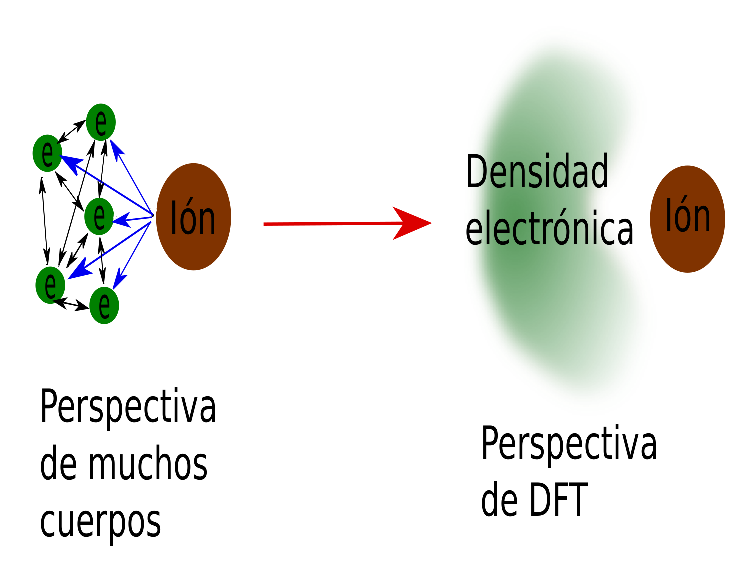
\epsfig{file=figuras/perspectivaDFT.eps, width=10.0cm,height=8.0cm}
  	\caption{idea de la teor\'ia funcional de la densidad que consiste en sustituir las interacciones de muchos cuerpos con una interacci\'on promedio por medio de la densidad electr\'onica.}
  	\label{im:dftIdea}
  \end{figure}
  
  La teor\'ia desarrollado por Hohenberg y Kohn realizaron una formulaci\'on de DFT como una teor\'ia exacta de un sistema de muchos cuerpos aunque solo para su estado base, por lo tanto  es importante encontrar los valores de expectaci\'on para los estados base $\Psi_0$ para la energ\'ia, la densidad y la densidad de la magnetizaci\'on  (ecs. \ref{ec:energia}, \ref{ec:denspin} y \ref{ec:magn}, respectivamente), es importante separar el Hamiltoniano  de la ecuaci\'on \ref{ec:shelectron} como:
  \begin{equation}
  \hat{H} =\hat{H}_0 + \hat{H}_{ext} \label{ec:sepHamilton}
  \end{equation}
  en donde $\hat{H}_0 = \hat{T}+\hat{V}_{int}$ y $\hat{H}_{ext}= \hat{V}_{ext} + E_{II}$,  cuando se desea considerar el aporte de la magnetizaci\'on, es necesario agregar una interacci\'on de estilo Zeeman de un campo magn\'etico externo con el sistema:
  \begin{equation*}
  -\pmb{B}_{ext} (\pmb{r}) \pmb{m} (\pmb{r})
  \end{equation*}  
  este potencial es valido debido a que solo se considera el aporte de la magnetizaci\'on de el spin y se puede considerar el potencial de interacci\'on debido a fuentes externas como 
  \begin{equation}
  \hat{H}_{ext} = \hat{V}_{Ex}^{s', s} = \hat{V}_{ext} \delta_{s',s} - \pmb{B}_{ext} (\pmb{r}) \pmb{m} (\pmb{r}) +E_{II} \label{ec:intExt}
  \end{equation}
  es importante notar que en caso de que se trabaje con una orientaci\'on no colineal es necesario agregar el t\'ermino de acople spin-\'orbita al campo magn\'etico externo:
  \begin{equation*}
  \pmb{B}_{ext} (\pmb{r}) \to  \pmb{B}_{ext} (\pmb{r}) + \frac{i \hbar^2}{\mu_{B} (2 m c)^2} \{[\nabla V_{ext}]\times \nabla \}
  \end{equation*}
  \newline
  La teor\'ia desarrollada muestra que el funcional de la energ\'ia est\'a caracterizado por la densidad de electrones (ec. \ref{ec:densidadr}) y la magnetizaci\'on (ec. \ref{ec:magn}):
  \begin{equation}
  E=E_{V_{ext}, \pmb{B}_{ext}} [n,\pmb{m}] \label{ec:func1}
  \end{equation}
  el primer teorema de Hohenberg y Kohn se relaciona con el hecho  de que el potencial externo dado por la ecuaci\'on \ref{ec:intExt}  est\'a determinado \'unicamente por la densidad y la magnetizaci\'on en el estado base $n_0$ y $\pmb{m}_0$, esto se muestra en la figura \ref{fig:hk1}.
  \begin{figure}[!hbt]
  	\centering
  	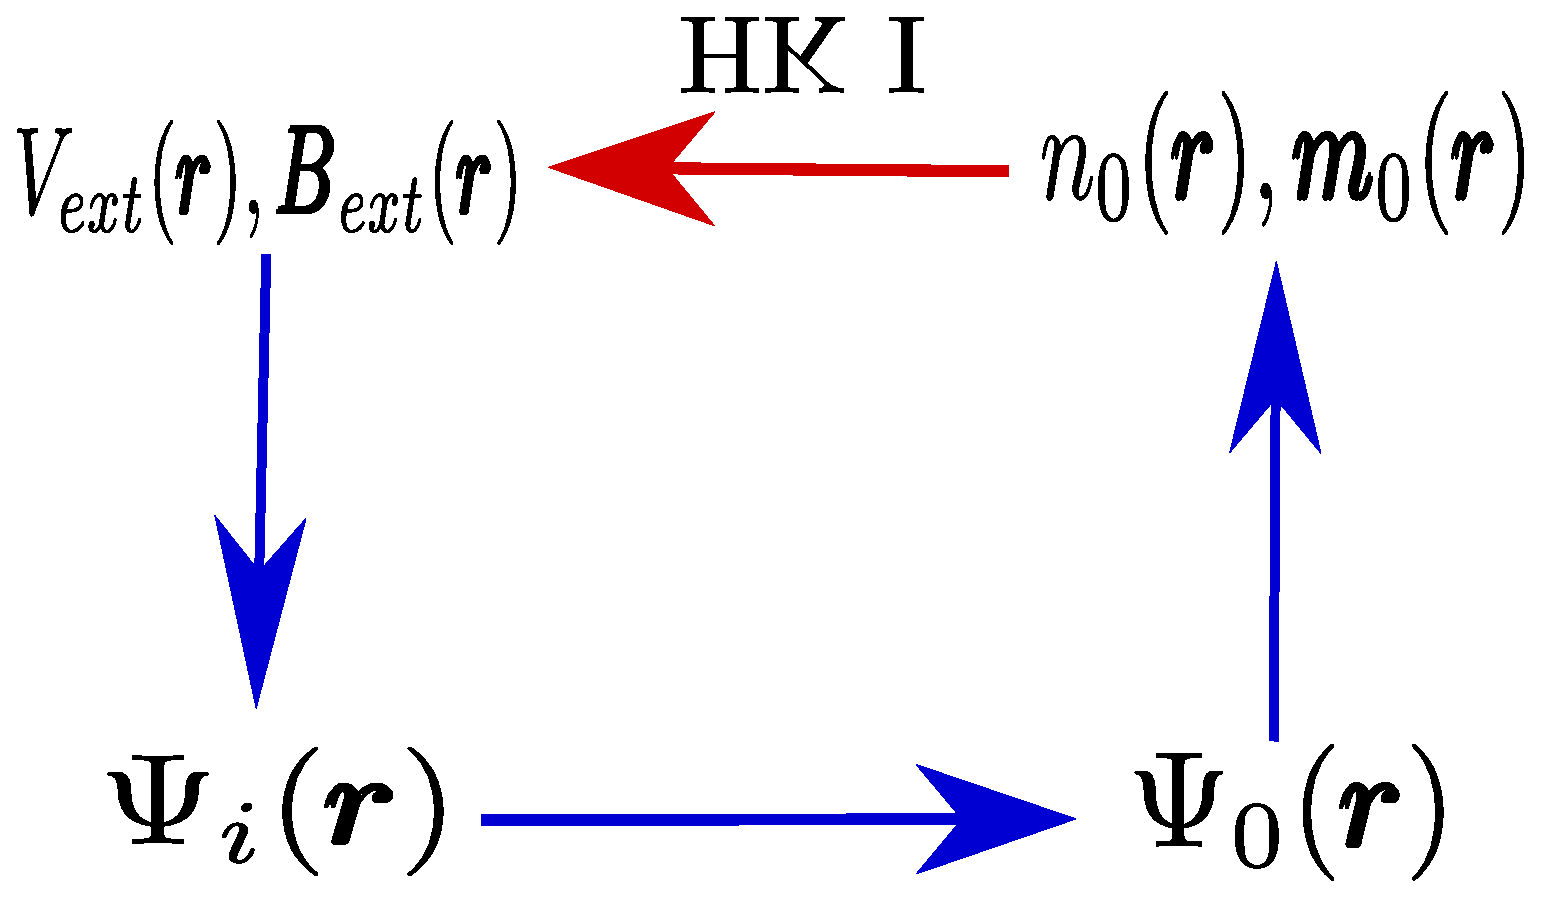
\epsfig{file=figuras/HK1.eps, width=8.0cm,height=5.0cm}
  	\caption{Representaci\'on esquem\'atica del primer teorema de Hohenberg-Kohn}
  	\label{fig:hk1}
  \end{figure}
\newline
  En la figura \ref{fig:hk1} las flechas azules muestran la soluci\'on que usualmente se sigue para resolver la ecuaci\'on de schr\"odringer y la flecha roja indica la relaci\'on establecida por el primer teorema de Hohenberg-Kohn,  como consecuencia de este teorema, dos estados base distintos $\Psi_0 $ y $\Psi_0 '$ dan lugar a dos matrices de densidad de spines diferentes $n_{s',s} \not =n_{s',s}' $ y por lo tanto $n(\pmb{r}), \pmb{m}(\pmb{r}) \not = n'(\pmb{r}), \pmb{m}'(\pmb{r})$, debido a este teorema es posible determinar las funciones de muchos cuerpos para todos los niveles sin importar que est\'en desocupados, entonces todas las propiedades del sistema se pueden determinar teniendo s\'olo la densidad de electrones en el estado base.
  \newline
  El segundo teorema se relaciona con que es posible determinar un funcional para la energ\'ia $E_{V_{ext}, \pmb{B}_{ext}}[n,\pmb{m}]$ en t\'erminos de la densidad y la magnetizaci\'on que es v\'alido para cualquier potencial externo $\hat{V}_{Ex}^{s', s}$. Para un $\hat{V}_{Ex}^{s', s}$ particular , la energ\'ia del estado base del sistema es el m\'inimo global de este funcional y la densidad $n(\pmb{r})$ y la magnetizaci\'on $\pmb{m}(\pmb{r})$ que minimizan el funcional son los par\'ametros exactos para el estado base  $n_0(\pmb{r})$ y $\pmb{m}_0(\pmb{r})$, el potencial puede ser escrito como:
  \begin{equation}
   E_{V_{ext}, \pmb{B}_{ext}}[n,\pmb{m}]= F[n,\pmb{m}] + \int d \pmb{r} \{V_{ext} (\pmb{r}) n(\pmb{r})+\pmb{B}_{ext} (\pmb{r}) \pmb{m} (\pmb{r}) \} +E_{II} \label{ec:funcional}
  \end{equation}
  en donde$F[n,\pmb{m}]$ es el llamado funcional universal el cual incluye las energ\'ias cin\'eticas y potencial del sistema de electrones:
  \begin{eqnarray}
  F[n,\pmb{m}]&= \langle \Psi_0 [n,\pmb{m}]| \hat{T}+\hat{V}_{int} | \Psi_0 [n,\pmb{m}] \rangle \nonumber \\
              &= T[n,\pmb{m}] + V_{int} [n,\pmb{m}] \label{ec:funcF}
  \end{eqnarray}
  
  para un potenciales externo  fijos, la densidad $n_0 (\pmb{r})$ y la magnetizaci\'on $\pmb{m}_0 (\pmb{r})$, la energ\'ia del estado base 
  \begin{equation}
  E_0= E_{V_{ext}, \pmb{B}_{ext}}[n_0,\pmb{m}_0] \label{ec:estadoBase}
  \end{equation}
  obedece la desigualdad
  \begin{equation}
  E_0 < E_{V_{ext}, \pmb{B}_{ext}}[n,\pmb{m}] \label{ec:desig}
  \end{equation}
  para $ n (\pmb{r}),\pmb{m} (\pmb{r}) \not = n_0 (\pmb{r}),\pmb{m}_0 (\pmb{r})$, de tal forma que es posible resumir el segundo  teorema de Hohenberg-Kohn como:
  \begin{equation}
  E_0 = \min_{n  \to n_0, \pmb{m} \to \pmb{m}_0} E_{V_{ext}, \pmb{B}_{ext}}[n,\pmb{m}]  \label{ec:HKII}
  \end{equation}
  Por consecuencia de este segundo teorema, el funcional de la ecuaci\'on \ref{ec:funcional} es suficiente para determinal la energ\'ia del estado base as\'i como su densidad y magnetizaci\'on, en la siguiente secci\'on se mostrar\'a el proceso general para encontrar estos valores por medio de las ecuaciones de Kohn-Sham adem\'as que se mostrar\'a la raz\'on por la que se les llama evaluaci\'on auto consistente.
  
  \section{Ecuaciones de Kohn-Sham}
  Dado  que los teoremas vistos en la secci\'on anterior establecen de forma rigurosa que solo se necesita conocer la densidad y la magnetizaci\'on para conocer la energ\'ia en el estado base de un sistema de muchos cuerpos, en un principio esto ser\'ia suficiente para desarrollar una teor\'ia funcional de la densidad pero no es posible implementarlo num\'ericamente, es as\'i como surge la teor\'ia desarrollada  por  Kohn y Sham, la cual es crear un sistema de ecuaciones auxiliar para resolver el problema de muchos cuerpos que representa el Hamiltoniano de la ecuaci\'on \ref{ec:sh}, ellos propusieron que la densidad y la magnetizaci\'on del estado base son igual a los valores de alg\'un sistema libre de interacci\'on, este esquema se basa en asumir que el estado base del sistema de muchos cuerpos la densidad y la magnetizaci\'on pueden ser representadas en un sistema auxiliar para part\'iculas sin interacci\'on y el hamiltoniano auxiliar se elige de tal forma que el operador de la energ\'ia cin\'etica $ \hat{T}$ y el potencial local $ V_{eff}^s $ act\'uan en un electr\'on con spin $s$ en la posici\'on $\pmb{r}$. Tal Hamiltoniano del sistema auxiliar se puede escribir como (Utilizando unidades de Hartree):
  \begin{equation}
  \hat{H}_{aux}^{s} = - \frac{1}{2} \nabla^2 + V_{eff}^s (\pmb{r}) \label{ec:HAux}
  \end{equation}  
  si se considera un sistema de spines colineales, se dice que el n\'umero de electrones independientes es $N = N_{\uparrow}+ N_{\downarrow}$, la densidad de electrones en este sistema est\'a dada por la ecuaci\'on \ref{ec:denspin} con $s' = s$:
  \begin{equation}
  n_s (\pmb{r}) = \sum_{i} n_{i,s} |\psi_{i,s } (\pmb{r})|^2 \label{ec:den1spin}
  \end{equation}
  de tal forma que la energ\'ia cin\'etica de una sola part\'icula $T_sp$ se define como:
  \begin{equation}
  T_{sp} = -\frac{1}{2} \sum_{s} \sum_{i} n_{i,s} \int d^3 r ~\psi_{i,s }^* (\pmb{r}) \nabla^2 \psi_{i,s } (\pmb{r})  = \frac{1}{2} \sum_{s} \sum_{i} n_{i,s} \int d^3 r  |\nabla \psi_{i,s } (\pmb{r}) |^2 \label{ec:funCinetica}
  \end{equation}
   adem\'as hay que tomar en cuenta la interacci\'on entre part\'iculas entre part\'iculas como la de Hartree (ec. \ref{ec:Hartree}), entonces se puede reescribir el funcional de la ecuaci\'on \ref{ec:funcional} sin considerar campos magn\'eticos externos como: 
   \begin{equation}
   E_{KS}[n] = T_{sp}[n]+ \int d \pmb{r} V_{ext} (\pmb{r}) n_s (\pmb{r}) +E_{Hartree} [n] + E_{XC}^s [n] + E_{II} \label{ec:funcHK}
   \end{equation}
   todos los efectos de intercambio y correlaci\'on se agrupan en $E_{XC}^s [n]$ el cual se puede escribir en t\'erminos del funcional de Hohenberg-Kohn (ec. \ref{ec:funcional}) :
   \begin{equation}
   E_{XC}^s [n] = F[n]-(T_{sp} [n]+E_{Hartree}[n]) \label{ec:eXC2}
   \end{equation}
   la cual se puede reescribir como:
   \begin{equation}
   E_{XC}^s [n]= \langle \hat{T} \rangle - T_{sp} [n]+\langle \hat{V}_{int} \rangle-E_{Hartree} [n] \label{ec:Exc2}
   \end{equation}
   la cual si se compara con la ecuaci\'on \ref{ec:energiaXC} se puede notar que la energ\'ia de intercambio y correlaci\'on no solo depende de la diferencia entre las interacciones Coulombicas ($\langle \hat{V}_{int} \rangle-E_{Hartree}[n]$) sino tambi\'en por la diferencia entre la energ\'ia cin\'etica entre el sistema con interacciones y el que no las tiene ($ \langle \hat{T} \rangle - T_{sp} [n] $).
   \newline
   Para cumplir con el segundo teorema de Hohenberg y Kohn se minimiza el funcional de la energ\'ia (ec. \ref{ec:funcHK}) con respecto  a las funciones de los orbitales $\psi_{i,s } $: 
   \begin{equation}
   \frac{\delta E_{KS} [n_s]}{\delta \psi_{i,s } ^* (\pmb{r})}= \frac{\delta T_{sp} }{\delta \psi_{i,s } ^* (\pmb{r}) } + \left[\frac{\delta E_{ext}}{\delta n_s (\pmb{r})}+\frac{\delta E_{Hartree}}{\delta n_s (\pmb{r})}+  \frac{\delta E_{XC}^s}{\delta n_s (\pmb{r})}\right] \frac{\delta n_s (\pmb{r})}{\delta \psi_{i,s } ^* (\pmb{r})} =0 \label{ec:ecEulerFun}
   \end{equation}
   Utilizando las ecuaciones \ref{ec:den1spin} y \ref{ec:funCinetica} se obtiene lo siguiente:
   \begin{equation}
   \frac{\delta T_{sp} }{\delta \psi_{i,s } ^* (\pmb{r}) }= -\frac{1}{2} \nabla^2 \psi_{i,s } (\pmb{r}); ~~ \frac{\delta n_s (\pmb{r})}{\delta \psi_{i,s } ^* (\pmb{r})}= \psi_{i,s } (\pmb{r}) \label{ec:simp}
   \end{equation} 
   Utilizando las ecuaciones \ref{ec:ecEulerFun} y  \ref{ec:simp} se utiliza el m\'etodo de los multiplicadores de Lagrange  sujeto a la condici\'on $\langle \psi_{i,s} | \psi_{j,s'} \rangle =   \delta_{i,j}\delta_{s',s}$   para obtener la ecuaci\'on de Kohn-Sham  :
   \begin{equation}
   (H_{KS}^s -\epsilon_{i,s})\psi_{i,s } (\pmb{r}) = 0 \label{ec:ShKS}
   \end{equation}
   con los eigenvalores $\epsilon_{i,s} $   y $ H_{KS}^s $ es el hamiltoniano efectivo definido por:
   \begin{equation}
    H_{KS}^s = -\frac{1}{2} \nabla^2 + V_{KS}^s (\pmb{r}) \label{ec:HamiltonianoKS}
   \end{equation}
   con
   \begin{eqnarray}
     V_{KS}^s (\pmb{r}) &=& V_{ext} (\pmb{r})+  \frac{\delta E_{Hartree}}{\delta n_s (\pmb{r})}+  \frac{\delta E_{XC}^s}{\delta n_s (\pmb{r})} \nonumber \\
      &=& V_{ext} (\pmb{r})+ V_{Hartree} (\pmb{r}) + V_{XC}^s (\pmb{r}) \label{ec:potKS} 
   \end{eqnarray}
   las ecuaciones \ref{ec:ShKS}-\ref{ec:potKS} son las ecuaciones de Kohn-Sham que tienen la forma de ecuaciones de part\'iculas independientes las cuales tienen que ser resueltas autoconsistentemente con el c\'alculo de la densidad (ec. \ref{ec:den1spin}) y la energ\'ia total (ec. \ref{ec:funcHK}), la evaluaci\'on no autoconsistente para el caso de spines colineales se muestra en la figura \ref{fig:esq}, en este caso se tienen que resolver para dos orientaciones de spines $\uparrow, \downarrow$, el proceso inicia calculando la densidad de electrones considerando que los \'atomos est\'an aislados, despu\'es se compara la energ\'ia de kohn-Sham con la iteraci\'on anterior, si la diferencia es casi cero entonces se dice que el calculo de energ\'ia converge y termina la ejecuci\'on, en caso contrario se vuelve a calcular la densidad con las funciones de onda calculadas anteriormente y se repite el proceso. 
   \begin{figure}[!hbt]
   	\centering
   	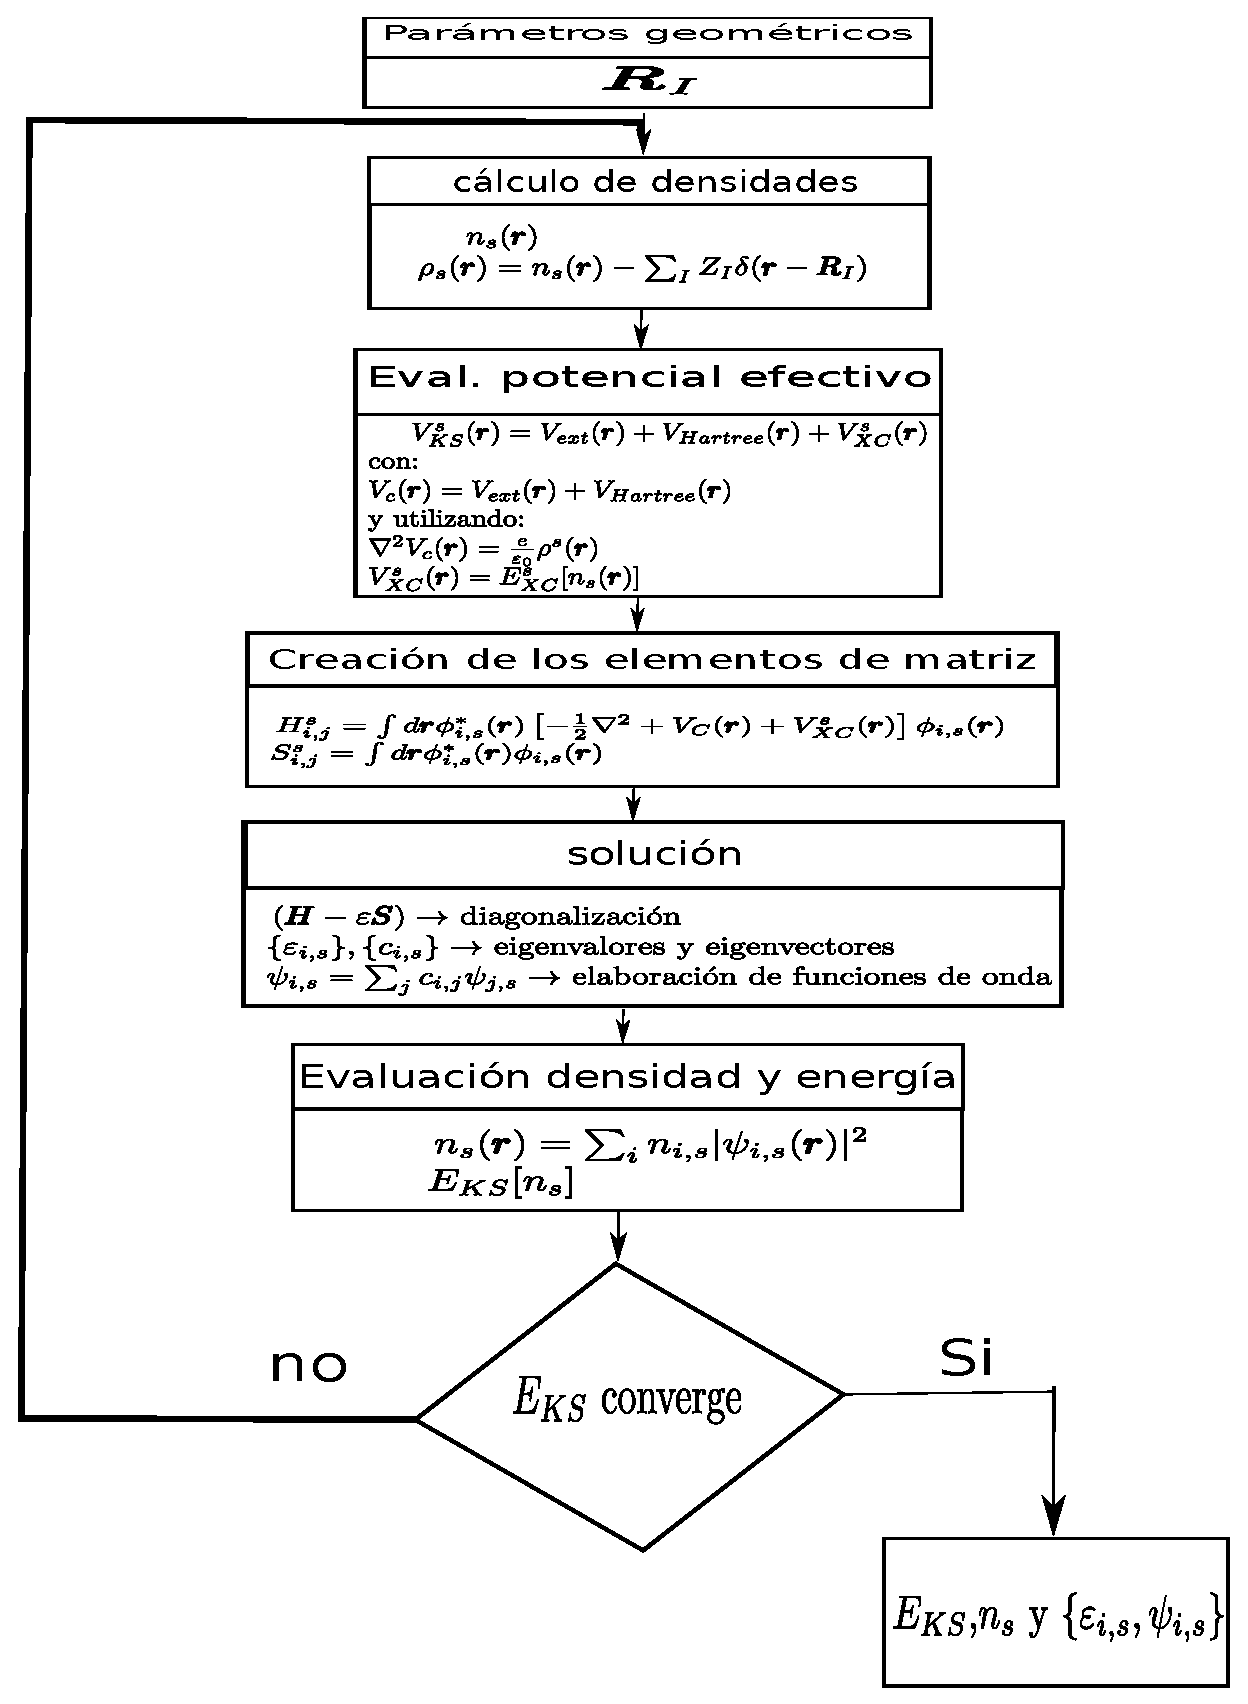
\epsfig{file=figuras/diagramaAuto.eps, width=10.0cm,height=18.0cm}
   	\caption{ciclo autoconsistente de la soluci\'on de las ecuaciones de Kohn-Sham de spines colineales}
   	\label{fig:esq}
   \end{figure}
   \newline
   En el caso de los spines no colineales, no es posible separar la funci\'on de onda tal como se hizo en la secci\'on \ref{sec:introdft},$\phi_{\Lambda} (\pmb{r},s)\not = \psi_{i,s } (\pmb{r}_j) \alpha_i (s_j) $, con $\Lambda$ representando los n\'umeros cu\'anticos  del orbital, los cuales se ven influenciados por el acople spin-\'orbita, tambi\'en es necesario agregar un campo magn\'etico de intercambio y correlaci\'on:
   \begin{equation*}
   B_{XCj} (\pmb{r}) = - \frac{\delta E_{XC} [n,\pmb{m}]}{\delta m_j (\pmb{r})}
   \end{equation*}
   el cual representa un campo magn\'etico interno inducido por  debido a los efectos de intercambio y correlaci\'on y el cual tiene consecuencias interesantes sobre ls part\'iculas, en lugar de un sistema de dos ecuaciones representadas por la ecuaci\'on \ref{ec:ShKS} para el caso colineal se tiene que resolver un sistema de cuatro ecuaciones para el caso no colineal:
   \begin{multline}
   \sum_{s}  \left[-\frac{1}{2} \nabla^2 + V_{ext} (\pmb{r})+ V_{Hartree} (\pmb{r}) + V_{XC} (\pmb{r}) \right] \delta_{s',s}  \phi_{\Lambda} (\pmb{r},s)\\ - \mu_{B} \sum_{s}  [\pmb{B}_{ext} (\pmb{r})+ \pmb{B}_{XC} (\pmb{r}) ] \pmb{\sigma_{s,s'}} \phi_{\Lambda} (\pmb{r},s) = \varepsilon_{\Lambda} \phi_{\Lambda} (\pmb{r},s) \label{ec:KSnoColl}
   \end{multline}
   en donde $s$ toma los valores de $\uparrow, \downarrow$ y los dos las dos componentes del spinor, adem\'as hay que considerar el acople spin \'orbita tal como se dijo en la secci\'on \ref{sec:Ho-Ko}.
   \subsection{Evaluaci\'on no auto consistente}
   Cuando es necesario calcular estructuras de bandas,  densidad de estados entre otros, se utiliza una red mas densa en el espacio rec\'iproco (de esta red se habla en la secci\'on \ref{sec:solespacioK}), entonces se realiza un ca\'alculo qu no es auto consistente, es decir no se realiza el ciclo ilustrado en la figura \ref{fig:esq}, el proceso consiste en tomar la densidad de carga obtenida por la evaluaci\'on auto consistente  y resolver la ecuaciones de Kohn-Sham (ecs. \ref{ec:ShKS}-\ref{ec:potKS}) de tal forma que se obtiene una nueva densidad $n_0$ en base a los egenvalores que se obtuvieron de la resoluci\'on  de las ecuaciones de Kohn-Sham, con los eigenvalores que se obtienen es posible definir la energ\'ia de banda:
   \begin{equation}
   E_{banda} = \sum_{i} \varepsilon_{i,s} \label{ec:Eband}
   \end{equation}
   en donde s\'olo se suman los eigenvalores de los estados ocupados. En lugar de calcular la energ\'ia con ef funcional de Kohn-Sham (ec. \ref{ec:funcHK}) se utiliza el funcional de Harris:
   \begin{equation}
   E_{Harris} [n_0] = \sum_{i} \varepsilon_i - \int d^3 r V_{ext} [n_0] n_0 (\pmb{r}) - \frac{1}{2} \int d^3 r V_{Hartree} [n_0] n_0 (\pmb{r}) + E_{XC} [n_0] \label{ec:FuncHarris}
   \end{equation} 
   tal funcional tiene como caracter\'istica que var\'ia menos que el potencial de Kohn-Sham si se desplaza la densidad del estado base.
   \section{funconal de intercambio y correlaci\'on ($E_{XC} $)}\label{sec2:xc}
   Como se ha dicho en las secciones anteriores una parte fundamental de las ecuaciones de kohn-Sham es el potencial de intercambio y correlaci\'on, este funcional puede ser formulado en t\'erminos de la densidad de spin y de la posici\'on, existen diversas formas de aproximar este funcional, en especial se ver\'a la aproximaci\'on de gradientes generalizados la cual incluye gradientes de la densidad, adem\'as de que existen distintos funcionales tales como PW91,PBE,PBEsol, etc, en el presente trabajo se utiliz\'o el funcional PBE, el cual se tratar\'a en la secci\'on \ref{susec:PBE} despu\'es de presentar las principales caracter\'isticas del funcional exacto de $E_{XC}$ en la secci\'on \ref{susec:exXC}. 
   \subsection{Propiedades del funcional $E_{XC} $ exacto } \label{susec:exXC}
   Como se vio en la secci\'on \ref{sec:Ho-Ko}, el funcional del a energ\'ia de intercambio y correlaci\'on (ec. \ref{ec:Exc2} ) contiene contribuciones de la diferencia entre las energ\'ias cin\'eticas de los sistemas con y sin interacci\'on $(T-T_{sp})$ de tal forma que es necesaria una generalizaci\'on de la expresi\'on dada en la ecuaci\'on \ref{ec:energiaXC}, aunque $E_{XC}$ continua siendo un funcional de la densidad que puede ser escrito por:
   \begin{equation}
   E_{XC}^s [n_s] = \int d \pmb{r} n_s (\pmb{r}) \epsilon_{XC} (\pmb{r}; [n_s]) \label{ec:enGenXCf}
   \end{equation} 
   donde $ \epsilon_{XC} (\pmb{r}; [n_s])$ es la energ\'ia de intercambio y correlaci\'on por part\'icula en pa posici\'on $\pmb{r}$ que depende solo de la densidad $n_s$ , en el caso de que los spines no est\'en orientados colinealmente, en principio se tiene que considerar la magnetizaci\'on y la polarizaci\'on.
   \newline
   Para analizar la contribuci\'on de $E_{XC} $ en el funcional de energ\'ia \ref{ec:funcHK} se utiliza el m\'etodo llamado de conexi\'on adiab\'atica, el cual es una generalizaci\'on del teorema de Hellman-Feymann (que se tratar\'a mas adelante), el cual dice que el cambio de la energ\'ia del sistema con respecto al par\'ametro $\lambda$ es igual al elemento de matriz de la derivada del Hamiltoniano con respecto al mismo par\'ametro, entonces una diferencia de energ\'ia entre dos estados $\lambda_1$ y $\lambda_2$ puede ser calculada como una integral sobre una variaci\'on continua del Hamiltoniano de  $\lambda_1$ a $\lambda_2$. El nombre de conexi\'on adiab\'atica se debe a que se asume que el Hamiltoniano que conecta los dos estados est\'a en el estado base para cada valor de $\lambda$. Las expresiones generales est\'an dadas por:
   \begin{equation}
   \frac{\partial E_0}{\partial \lambda} = \frac{\partial}{\partial \lambda} \left \langle \Psi_0^{\lambda} \left | \hat{H}_0 ^{\lambda} \right |  \Psi_0^{\lambda} \right \rangle = \left \langle \Psi_0^{\lambda} \left | \frac{\partial \hat{H}_0 ^{\lambda}}{\partial \lambda} \right |  \Psi_0^{\lambda} \right \rangle \label{ec:adAproxderivada}
   \end{equation}  
   o escrito en forma de integral:
   \begin{equation}
   \Delta E_0 = \int_{\lambda_1}^{\lambda_2} d \lambda~ \frac{\partial E_0}{\partial \lambda} = \int_{\lambda_1}^{\lambda_2} d \lambda \left \langle \Psi_0^{\lambda} \left | \frac{\partial \hat{H}_0 ^{\lambda}}{\partial \lambda}  \right |  \Psi_0^{\lambda} \right \rangle \label{ec:adAproxInt}
   \end{equation}
   Entones lo que se hace es escalar el t\'ermino de la interacci\'on entre electrones $\lambda \hat{V}_{int}$ con el par\'ametro $\lambda (0 \le \lambda \le 1)$ entre un sistema sin interacci\'on y uno con interacci\'on, tambi\'en se asume que $n(\pmb{r})= n^{\lambda} (\pmb{r})$ se puede fijar al mismo valor a pesar de las interacciones, entonces es posible definir el siguiente Hamiltoniano en ligar del de la ecuaci\'on \ref{ec:shelectron} como: 
   \begin{equation}
   \hat{H}_{0}^{\lambda} = \hat{T}+ \hat{V}_{ext}^{\lambda}+ \lambda \hat{V}_{int} \label{ec:SH1Elec}
   \end{equation}
   en donde se reemplaza el potencial externo $\hat{V}_{ext} $ con $\hat{V}_{ext}^{\lambda} $ el cual garantiza que no cambie la densidad. utilizando las ecuaciones \ref{ec:adAproxderivada} y \ref{ec:adAproxInt}, entonces se puede esccribir el funcional de la energ\'ia del estado base (ec. \ref{ec:funcional} con $\pmb{B}_{ext}=0$):
   \begin{subequations}
   	\begin{equation*}
   	E_0 = E_{V_{ext}} [n] = \langle \Psi_0^1 | \hat{H}_0 ^ 1 | \Psi_0^1 \rangle
   	\end{equation*}
   	\begin{equation*}
   	=\langle \Psi_0^0 | \hat{H}_0 ^ 0 | \Psi_0^0 \rangle + \int_{0}^{1} d \lambda \frac{\partial}{\partial \lambda } \left \langle \Psi_0^{\lambda} \left | \hat{H}_0 ^{\lambda} \right |  \Psi_0^{\lambda} \right \rangle
   	\end{equation*}
   	\begin{equation*}
   	=\langle \Psi_0^0 | \hat{H}_0 ^ 0 | \Psi_0^0 \rangle + \int d \pmb{r} [V_{ext}^1 (\pmb{r})-V_{ext}^0 (\pmb{r})] n (\pmb{r}) + \int_{0}^{1} d \lambda  \left \langle \Psi_0^{\lambda} \left | \hat{V}_{int} \right |  \Psi_0^{\lambda} \right \rangle
   	\end{equation*}
   \end{subequations}
   y asumiendo  que $V_{ext}^1 (\pmb{r}) \equiv V_{ext} (\pmb{r})$:
   \begin{equation*}
   E_0 = E_{V_{ext}} [n]= \langle \Psi_0^0 | \hat{T} | \Psi_0^0 \rangle + \int d \pmb{r} V_{ext} (\pmb{r}) n (\pmb{r}) + \int_{0}^{1} d \lambda  \left \langle \Psi_0^{\lambda} \left | \hat{V}_{int} \right |  \Psi_0^{\lambda} \right \rangle
   \end{equation*}
   dado que el primer t\'ermino corresponde a $T_{sp}$ se puede encontrar en lugar de \ref{ec:Exc2} la siguiente expresi\'on:
   \begin{equation}
   E_{XC} [n] = \int_{0}^{1} d \lambda  \left \langle \Psi_0^{\lambda} \left | \hat{V}_{int} \right |  \Psi_0^{\lambda} \right \rangle-E_{Hartree} = \frac{1}{2} \int d \pmb{r} n(\pmb{r})\int d \pmb{r'}  \frac{\widetilde{n }_{xc}(\pmb{r},\pmb{r'})}{|\pmb{r}-\pmb{r'}|} \label{ec:Exc3}
   \end{equation}
   en donde $\widetilde{n }_{xc} (\pmb{r},\pmb{r'})$ es la constante de acople de un hueco promediado
   \begin{equation}
   \widetilde{n }_{xc} (\pmb{r},\pmb{r'}) = \int_{0}^{1} d \lambda n_{xc}^{\lambda} (\pmb{r},\pmb{r'}) \label{ec:avHole}
   \end{equation}
   junto con las ecuaciones \ref{ec:enGenXCf} y \ref{ec:Exc3} es posible escribir la energ\'ia de intercambio y correlaci\'on por part\'icula $\epsilon_{XC} $ como:
   \begin{equation}
   \epsilon_{XC} (\pmb{r}; [n])= \frac{1}{2} \int d \pmb{r'}  \frac{\widetilde{n }_{xc}(\pmb{r},\pmb{r'})}{|\pmb{r}-\pmb{r'}|} \label{ec:densEXC}
   \end{equation}
   debido a estas ecuaciones, es posible definir a la energ\'ia de intercambio y correlaci\'on como la energ\'ia  de intercambio y correlaci\'on de un hueco promediada de un caso sin interacci\'on $\lambda=0$ a un sistema con interacci\'on $\lambda=1$. Dado que la densidad es constante en todo lugar si $\lambda$ cambia entonces $\epsilon_{XC} (\pmb{r}; [n]) $ es un funcional de la densidad en todo el espacio, entonces $E_{XC} [n]$ se puede considerar como una interpolaci\'on entre un caso en donde s\'olo existe energ\'ia de intercambio y otro en donde es completamente una energ\'ia de correlaci\'on.  Se puede expresar el potencial de intercambio y correlaci\'on en funci\'on de la energ\'ia de intercambio y correlaci\'on por part\'icula:
   \begin{equation}
   V_{XC} (\pmb{r}) = \epsilon_{XC} (\pmb{r}; [n]) + n(\pmb{r}) \frac{\delta \epsilon_{XC} (\pmb{r}; [n])}{\delta n(\pmb{r}) } \label{ec:potXC}
   \end{equation}  
   y la generalizaci\'on para el caso de spines colineales es la siguiente:
   \begin{equation}
   V_{XC}^s (\pmb{r}) = \epsilon_{XC} (\pmb{r}; [n]) + n(\pmb{r}) \frac{\delta \epsilon_{XC} (\pmb{r}; [n])}{\delta n_s(\pmb{r}) } \label{ec:potXCspin}
   \end{equation}
   en donde se toma en cuenta que $\epsilon_{XC} \equiv \epsilon_{XC} \left(\pmb{r}; \left[ n_{\uparrow}, n_{\downarrow} \right]\right) $ es un funcional de las dos densidades de spines.

   
   \subsection{Funcional gradientes generalizados, PBE} \label{susec:PBE}
   Una de las primeras aproximaciones que se realizaron a la energ\'ia de intercambio y correlaci\'on fue la aproximaci\'on local de la densidad (LDA por sus siglas en ingl\'es), la cual presenta errores tales como la sobre estimaci\'on de de las energ\'ias de cohesi\'on de casi todos ls s\'olidos adem\'as de la subestimaci\'on de los par\'ametros de red en varios casos as\'i como  los errores al momento de describir sistemas altamente correlacionados y en especial presenta problemas con \'atomos de metales de trancisi\'on, una forma de corregir estos errores es incluir correcciones de gradientes de la densidad de tal forma que la energ\'ia de intercambio y correlaci\'on puede ser escrita en funci\'on de un densidad de energ\'ia de intercambio y correlaci\'on $g_{r} [n]$:
   \begin{equation*}
   E_{XC} [n]= \int d^3~ r g_{r} [n]
   \end{equation*}
   y esta densidad se puede expandir en series:
   \begin{equation*}
   g_{r} [n] = g_0 (n(\pmb{r}))+ g_1 (n(\pmb{r})) [\nabla n(\pmb{r})]+ \ldots
   \end{equation*}
   esta idea fue propuesta por Kohn-Sham aunque esta no soluciona los principales problemas de LDA, por tal motivo se implement\'o la aproximaci\'on de gradientes generalizados (GGA por sus siglas en ingl\'es) cuya expresi\'on para la energ\'ia de intercambio y correlaci\'on est\'a dada por:
   \begin{multline}
      E_{XC}^{GGA} [n_{\uparrow} (\pmb{r}), n_{\downarrow}(\pmb{r})] = \int d^3 r ~ n(\pmb{r}) \epsilon_{XC} \left(n_{\uparrow} (\pmb{r}), n_{\downarrow}(\pmb{r}), \left|\nabla n_{\uparrow} (\pmb{r}) \right|^2, \left|\nabla n_{\downarrow} (\pmb{r}) \right|^2 \right)  \\
      = \int d^3 r ~ n(\pmb{r}) \epsilon_{X}^{hom} (n) F_{XC} \left(n_{\uparrow} (\pmb{r}), n_{\downarrow}(\pmb{r}), \left|\nabla n_{\uparrow} (\pmb{r}) \right|^2, \left|\nabla n_{\downarrow} (\pmb{r}) \right|^2 \right) \label{ec:funcXCGGA}
   \end{multline}
   en donde $ epsilon_{X}^{hom} (n) = -3k_F / 4\pi $ es la energ\'ia de intercambio pro part\'icula  de un gas de electrones homog\'eneo no polarizado en donde $k_F = (3 \pi^2 n)^{1/3}$ es el vector de onda de Fermi y $F_{XC}$ es una fucni\'on adimensional de las densidades y sus gradientes, tal funcional \ref{ec:funcXCGGA} es llamado funcional XC semilocal. Es importante recordar que es posible separar la parte puramente de correlaci\'on de la de intercambio de la siguiente manera: $ \epsilon_{XC} (\pmb{r}; [n] )= \epsilon_{X} (\pmb{r}; [n] )+ \epsilon_{C} (\pmb{r}; [n] ) $ y por lo tanto tambi\'en es v\'alido realizar la siguiente divisi\'on $ F_{XC} = F_{X}+ F_{C} $.
   \newline
   Una de las aproximaciones mas utilizadas es la desarrollada por Perdew, Burke y Enzerhof (PBE). La parte correspondiente a el intercambio puede ser escrita de la siguiente forma:
   \begin{equation}
   E_X [n_{\uparrow}, n_{\downarrow}]= \frac{1}{2} \left[E_{X} [2 n_{\uparrow}] + E_{X} [2 n_{\downarrow}]   \right] \label{ec:divEx}
   \end{equation}
   adem\'as se puede definir el gradiente de densidad reducida como:
   \begin{equation}
   s(\pmb{r})= \frac{|\nabla n (\pmb{r})|}{2 k_F n (\pmb{r}) } \label{ec:S}
   \end{equation}
   entonces es posible definir  $F_X (s)$ :
   \begin{equation}
   F_{X}^{PBE} = 1+\kappa -\frac{\kappa}{1+\mu s^2 /\kappa} \label{ec:F_X-PBE}
   \end{equation}
   donde $\mu = 0.21951 $ y $\kappa= 0.804 $. La energ\'ia de correlaci\'on est\'a dada por:
   \begin{equation}
   E_{C} ^{PBE} = \int d^3 r n \left\{\epsilon_{C}(r_s,\zeta)+ H^{PBE} (r_s,\zeta,t) \right\}\label{ec:funcCorr}
   \end{equation}
   donde $r_s = (3/4 \pi n)^{1/3}, ~ \zeta =(n_{\uparrow}-n_{\downarrow})/n, t=|\nabla n|/2 k_s \phi n, \phi= \frac{1}{2} [(1+\zeta)^{2/3}+(1-\zeta)^{2/3}], k_s = (4 k_F/\pi)^{1/2}$,
   \begin{equation}
   H^{PBE} = \gamma \phi^3 \ln \left\{1+ \frac{\beta}{\gamma} t^2 \left[\frac{1+At^2}{1+At^2+A^2 t^4}\right]\right\}, \label{ec:PBEH}
   \end{equation}
   \begin{equation}
   A=\frac{\beta}{\gamma} [exp\{-\epsilon_{C}^{hom}/\gamma \phi^3 \}-1]^{-1} \label{ec:A}
   \end{equation}
   y $\gamma=0.031091, ~\beta=0.066725$. Los gradientes reducidos $s$ y $t$ miden que tn r\'apido $n(\pmb{r})$ var\'ia en las escalas de la longitud de onda de Fermi $2\pi/k_F$ y el apantallamiento de Thomas-Fermi $1/k_s$ respectivamente, esta clase de funcionales si mejoran los resultados obtenidos con LSDA.
   \newline
   Es posible calcular el potencial de intercambio y correlaci\'on encontrando el cambio $\delta E_{XC} [n]$ con respecto a un cambio  $\delta n$ y $\nabla \delta n$,
   \begin{equation}
   \delta E_{XC} [n] = \sum_{s} \int d \pmb{r} \left[\epsilon_{XC} + n \frac{\partial \epsilon_{XC}}{\partial n_s} + n \frac{\partial \epsilon_{XC}}{\partial \nabla n_s} \right]_{\pmb{r},s} \delta n_s(\pmb{r}) \label{ec:ecpotVXC_1}
   \end{equation}
   el termino dentro de los par\'entesis cuadrados se puede considerar el potencial pero no tiene la forma de un potencial local debido al \'ultimo t\'ermino, existen tres aproximaciones para manejar este t\'ermino, el primero es encontrar el potencial local $V_{XC}^s (\pmb{r})$ por interacci\'on parcial del \'ultimo  t\'ermino
   \begin{equation}
   V_{XC}^s (\pmb{r}) = \left[\epsilon_{XC}+\frac{\partial \epsilon_{XC}}{\partial n_s}- \nabla \left(n \frac{\partial \epsilon_{XC}}{\partial \nabla n_s}\right) \right] \label{ec:potXC_2}
   \end{equation}
   el cual es el mas usado pero tiene como desventaja que requiere derivadas de mayor orden para la densidad lo cual crea dificultades num\'ericas.
   \newline
   La segunda aproximaci\'on es usar un operador de la forma de la ecuaci\'on \ref{ec:potXC} directamente para modificar las ecuaciones de Kohn-Sham. Usando el hecho de que la densidad se puede escribir en t\'erminos de las funciones de onda $\psi_i$ , el elemento de matriz se puede escribir como:
   \begin{equation}
   \langle \psi_i |\hat{V}_{XC}| \psi_i \rangle = \int \left[\tilde{V}_{XC} \psi_i ^* \psi_i + \psi_i ^* \pmb{V}_{XC} \cdot \nabla \psi_i + (\pmb{V}_{XC} \cdot \nabla \psi_i^*) \psi_i \right] \label{ec:potXC_3}
   \end{equation}
   donde $\tilde{V}_{XC} = \epsilon_{XC} + n (\partial \epsilon_{XC}/ \partial n)$ y $\pmb{V}_{XC} = n (\partial \epsilon_{XC} / \partial \nabla n) $, esta forma es mas estable en t\'erminos num\'ericos pero requiere la inclusi\'on de operaciones vectoriales en la ecuaci\'on de Kohn-Sham lo cual incrementa la el trabajo computacional.
   \newline
   Finalmente, la segunda aproximaci\'on fue propuesta por White y Bird consiste en tratar $E_{XC}$ como una funci\'on de la densidad, los t\'erminos de de los gradientes son definidos por una definici\'on operacional en funci\'on de la densidad, entonces la ecuaci\'on \ref{ec:potXC} puede ser escrita usando la regla de la cadena:
   \begin{multline}
   \delta E_{XC} [n] = \sum_{s} \int d \pmb{r} \left[\epsilon_{XC} + n \frac{\partial \epsilon_{XC}}{\partial n_s} \right] \delta n_s (\pmb{r}) \\
   + \sum_{s} \int \int \int d \pmb{r} \int d \pmb{r'} n(\pmb{r}) \left[\frac{\partial \epsilon_{XC}}{\partial \nabla n_s} \right] ~ \frac{\delta \nabla n(\pmb{r'})}{\delta n(\pmb{r})} \delta n_s (\pmb{r}) \label{ec:potXC_4}
   \end{multline}
   donde $ (\delta n(\pmb{r'})/\delta n(\pmb{r}))$ denota una derivada funcional y tambi\'en se puede notar que la densidad est\'a dada por puntos discretos en una red $n(\pmb{r}_m)$ en donde el gradiente $\nabla n(\pmb{r}_m) $ puede ser  determinado de la siguiente forma:
   \begin{equation}
   	\nabla n(\pmb{r}_m)= \sum_{m} \pmb{C}_{m-m'} n(\pmb{r}_m) \label{ec:gradDisc}
   \end{equation}  
   de tal forma que la derivada funcional tiene la siguiente forma:
   \begin{equation}
   \frac{\delta \nabla n(\pmb{r}_m)}{\delta n(\pmb{r}_m')} \rightarrow \frac{\partial \nabla n(\pmb{r}_m)}{\partial n(\pmb{r}_m')} = \pmb{C}_{m-m'} \label{ec:gradCmm}
   \end{equation}
   en donde $\pmb{C}_{m} = \{ C_m ^x , C_m ^y , C_m ^z  \}$  es un vector en las coordenadas espaciales. Si se utilizan los coeficientes $\pmb{C}_m$ son diferentes de cero en un rango finito y variando $n_s (\pmb{r}_m)$ en la expresi\'on para $E_{XC}$ y utilizando la regla de la cadena:
   \begin{equation}
   V_{XC}^s (\pmb{r}_m) = \left[\epsilon_{XC}+n \frac{\partial \epsilon_{XC}}{\partial n}\right]_{\pmb{r}_m, s} + \sum_{s'} \left[ n \frac{\partial \epsilon_{XC}}{\partial |\nabla n|} ~\frac{\nabla n}{\partial |\nabla n|}\right] _{\pmb{r}_m', s} \pmb{C}_{m'-m} \label{ec:potVxc}
   \end{equation}
   esta expresi\'on para el potencial reduce los problemas num\'ericos asociados con la expresi\'on \ref{ec:potXC_2} sin utilizar operadores vectoriales como en la ecuaci\'on \ref{ec:potXC_3} adem\'as que se puede notar que $V_{XC}^s (\pmb{r}_m)$ es una funci\'on no local de $n_s (\pmb{r}_m)$.
   \section{formalismo  en el espacio K}\label{sec:solespacioK}
   Debido a que generalmente los problemas que se tratan son s\'olidos cristalinos entonces es conveniente  utilizar como funciones base a ondas planas para la expansi\'on de los eigenfunciones para las ecuaciones de kohn-Sham (ec. \ref{ec:HamiltonianoKS}), para un sistema  translacionalmente invariante las ondas planas est\'an dadas por
   \begin{equation}
   \phi_{\pmb{k},\pmb{G}} (\pmb{r})= \frac{1}{\sqrt{\Omega}} e^{i (\pmb{k}+\pmb{G})\pmb{r}} \label{ec:ondaplana}
   \end{equation}
   en donde $\Omega$ es el volumen del sistema y $\pmb{k} $ est\'a en la zona de Brillouin y $\pmb{G}$ est\'a en la red rec\'iproca, adem\'as este conjunto de ondas planas es ortonormal:
   \begin{equation}
   \int d \pmb{r} \phi_{\pmb{k},\pmb{G}}^* (\pmb{r}) \phi_{\pmb{k},\pmb{G}} (\pmb{r}) = \delta_{\pmb{k}, \pmb{k'}} \delta_{\pmb{G}, \pmb{G'}} \label{ec:PWorto}
   \end{equation} 
   y completo
   \begin{equation}
   \sum_{\pmb{k}} \sum_{\pmb{G}}  \phi_{\pmb{k},\pmb{G}} (\pmb{r}) \phi_{\pmb{k},\pmb{G}}^* (\pmb{r'}) = \delta (\pmb{r}- \pmb{r'}). \label{ec:PWComp}
   \end{equation}
   Para un sistema translacionalmente invariante cada eigenfunci\'on de Kohn-Sham $\psi_{v,\pmb{k},s }$ que cumple con el teorema de Bloch se puede expandir como:
   \begin{equation}
   \psi_{v,\pmb{k},s } (\pmb{r}) = \sum_{\pmb{G}} c_{v,\pmb{k},s } \phi_{\pmb{k},\pmb{G}} (\pmb{r}) \label{ec:basePW}
   \end{equation}
   en donde $v$ es el \'indice de la banda co  spin $s$. La densidad cumple con $n_s (\pmb{r}) = n_(s) (\pmb{r}+\pmb{R})$ y toma la siguiente forma:
   \begin{eqnarray}
   n_s(\pmb{r}) &=& \sum_{\pmb{G}} e^{-i \pmb{G} \pmb{r}} \tilde{n}_s (\pmb{G})  \label{ec:desnsiadK}\\
   \tilde{n}_s (\pmb{G}) &=& \frac{1}{\Omega} \sum_{v,\pmb{k}} n_{v,\pmb{k},s} \sum_{\pmb{G'}} c_{v,\pmb{k},s}^* (\pmb{G'}+\pmb{G}) c_{v,\pmb{k},s} (\pmb{G'}) \nonumber
   \end{eqnarray}
   y la ecuaciones de Kohn-Sham \ref{ec:ShKS} toman la siguiente forma:
   \begin{equation}
   \sum_{\pmb{G'}} \left\{ \left[\frac{1}{2} (\pmb{k}+ \pmb{G})^2 - \varepsilon_{v,s} (\pmb{k}) \right] \delta_{\pmb{G},\pmb{G'}} + V_{KS} ^ s (\pmb{G}-\pmb{G'}) \right\} c_{v,\pmb{k},s} (\pmb{G'}) =0 \label{ec:HKSRes}
   \end{equation} 
   con la energ\'ia de banda $\varepsilon_{v,s} (\pmb{k})$. los coeficientes de Fourier $V_{KS} ^ s (\pmb{G}-\pmb{G'})$ de un potencial local o no local son considerados.
   \newline
   El uso de ondas planas (ec. \ref{ec:basePW}) se puede interpretar como el uso de una red en el espacio rec\'iproco como se ilustra en la figura \ref{fig:a-espacioK}. Para grandes vol\'umenes $\Omega$ se necesita un gran n\'umero de ondas planas pero debido  a que se est\'a utilizando sistemas peri\'odicos se tiene que la cantidad de puntos $\pmb{k}$ en la zona de Brillouin est\'a dado por $\sum_{\pmb{k}} = \frac{\Omega}{(2 \pi )^3} \Omega_{BZ}$  en donde el volumen de la zona de Brillouin est\'a dado por $\Omega_{BZ} =\frac{(2 \pi )^3}{\Omega_0} $ en donde $\Omega_0$ es el volumen de la celda unitaria.
   
   \begin{figure}[!htb]
   	\centering
   	\subfigure[]
   	{
   		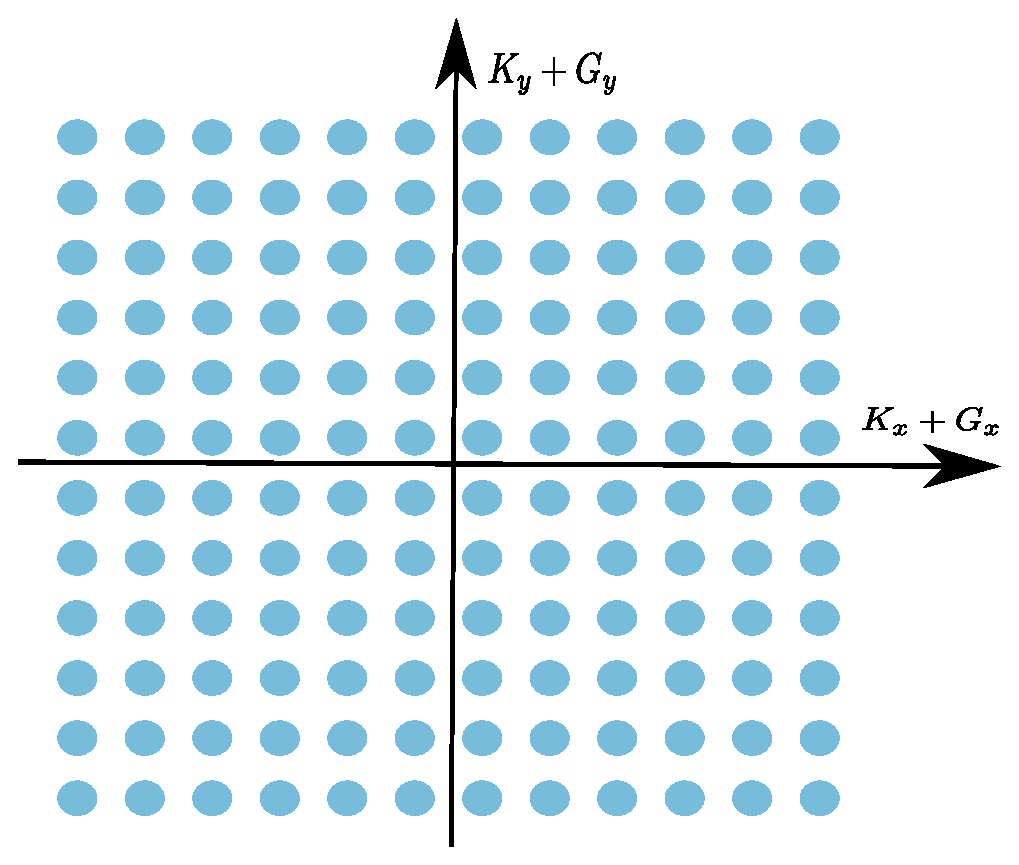
\epsfig{file=figuras/epacioKa.eps, width=5.0cm,height=5.0cm}
   		\label{fig:a-espacioK}
   	}
   \subfigure[]{
   	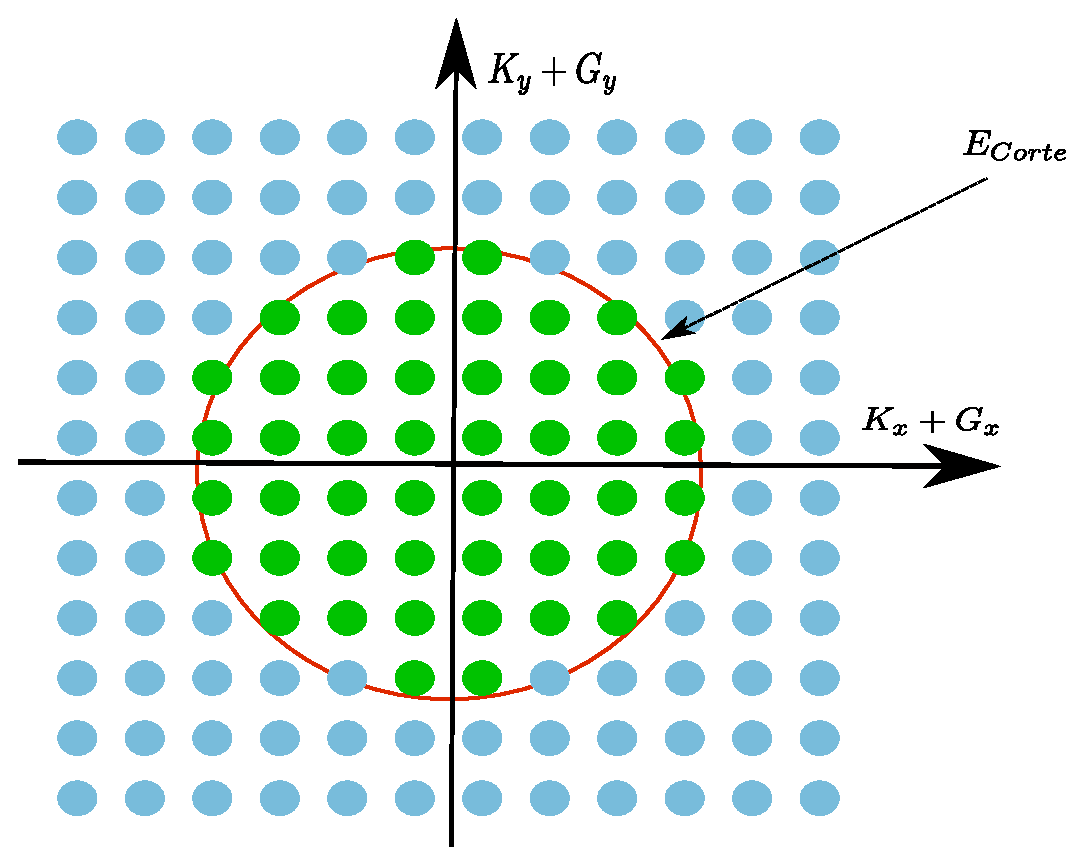
\epsfig{file=figuras/epacioKb.eps, width=5.0cm,height=5.0cm}
   	\label{fig:b-espacioK}
   }
   \caption{en la figura \ref{fig:a-espacioK} se muestra el mapeo en el espacio rec\'iproco usando ondas planas. En la figura \ref{fig:b-espacioK} e muestra c\'omo  se trunca el espacio rec\'iproco por medio de la energ\'ia de corte $E_{corte} $}
   \label{fig:espacioK}
   \end{figure}
   En la pr\'actica el n\'umero de ondas planas es limitado a una energ\'ia de corte $E_{corte}$ relacionada con la energ\'ia cin\'etica:
   \begin{equation}
   \int d \pmb{r}  \phi_{\pmb{k},\pmb{G}}^* (\pmb{r}) \left\{-\frac{1}{2} \nabla^2 \right\} \phi_{\pmb{k},\pmb{G}} (\pmb{r}) = \frac{1}{2} (\pmb{k}+ \pmb{G})^2 \le E_{corte}. \label{ec:Ecut}
   \end{equation}
   Esta energ\'ia determina el n\'umero de ondas planas que se usan en el c\'alculo y corresponda a truncar el espacio rec\'iproco como se muestra en la figura \ref{fig:b-espacioK} cuyo volumen es $\frac{4 \pi }{3} (2 E_{corte})^{3/2}$ entonces el n\'umero de ondas planas por \'atomo $N_{PW}$ es:
   \begin{equation}
   N_{PW}\cdot N_{atomo} \approx \frac{4 \pi }{3} \frac{(2E_{corte})^{3/2}}{\Omega_{BZ}}. \label{ec:NumAtomoPW}
   \end{equation}
   para muchos casos s\'olo se necesita una cantidad muy peque\~na de ondas planas tales como los \'atomos cuyos electrones de valencia pertenecen a los orbitales s y p si su comportamiento no se ve influido por los n\'ucleos. En el caso de que se contengan orbitales d se necesitar\'a una cantidad mayor de ondas planas debido a que estos estados est\'an mas localizados y por lo tanto se tienen que aumentar la energ\'ia de corte.
   \newline
   Importantes cantidades como la densidad y la energ\'ia total implican sumas en $\pmb{k}$ (o integrales sobre la zona de Brillouin ) en un principio se necesita un n\'umero infinito de puntos $\pmb{k}$ pero en la pr\'actica se utilizan un n\'umero finito de estos puntos resultando en un muestreo en la zona de Brillouin. El n\'umero de puntos depende de la dispersi\'on de las bandas ocupadas t\'ipicamente se necesitan mas puntos $\pmb{k}$ para metales. En el pasado se usaba la influencia de la simetr\'ia del sistema para obtener los puntos especiales $\pmb{k}^*$ en la zona irreducible de Brillouin, tales puntos eran suficientes para realizar tales sumas, posteriormente se desarroll\'o   un m\'etodo para obtener estos puntos desarrollado por Monkhorst y Pack que realiza un muestreo con puntos $\pmb{k}$ equidistantes con pesos id\'enticos
   \begin{equation}
   \pmb{k}_{n_1, n_2, n_3} = \sum_{i}^{3} \frac{2 n_i -N_i-1}{2N_i} \pmb{G}_i \label{ec:sampleMP}
   \end{equation}
   en donde $\pmb{G}_i $ son los vectores base del espacio rec\'iproco, $N_i$ es el n\'umero total de puntos en la direcci\'on $i$ y $n_i$ es el n]'umero de puntos \pmb{k} entre dos puntos en el espacio rec\'iproco conectados a trav\'es de  $\pmb{G}_i $.
    
   \section{C\'alculo de Fuerza} \label{sec:Fuerza}
   \subsection{Teorema de Hellman-Feynman} \label{subsec:HellFey}
   Este teorema es de gran importancia en la f\'isica y el cual fue formulado Hellman en 1932 y Feynman en 1939 deriv\'o el teorema para obtener una expresi\'on  para la fuerza  que se ejerce en un n\'ucleo est\'a dado estrictamente en t\'erminos de la densidad electr\'onica, independiente de la energ\'ia cin\'etica y de intercambio y correlaci\'on, este teorema tambi\'en es llamado "teorema de fuerza".
   \newline
   La fuerza puede ser escrita de la siguiente forma
   \begin{equation}
   \pmb{F}_I = - \frac{\partial E}{\partial \pmb{R}_I}. \label{ec:Fuerza}
   \end{equation} 
   Utilizando la expresi\'on general de la energ\'ia se obtiene la siguiente expresi\'on
   \begin{equation}
   -\frac{\partial E}{\partial \pmb{R}_I} = - \left\langle \Psi \left| \frac{\partial \hat{H}}{\partial \pmb{R}_I} \right| \Psi \right\rangle- \left\langle \frac{\partial \Psi}{\partial \pmb{R}_I} \left| \hat{H} \right| \Psi \right\rangle - \left\langle \Psi \left| \hat{H} \right|  \frac{\partial \Psi}{\partial \pmb{R}_I} \right\rangle - \frac{\partial E_{II}}{\partial \pmb{R}_I}. \label{ec:expansionF}
   \end{equation}
   Utilizando el hecho de que se est\'a en el estado base se conoce que este es un extremo por lo tanto los dos t\'erminos del medio de la ecuaci\'on \ref{ec:expansionF} son cero, entonces la expresi\'on para la fuerza (omitiendo el spin) es
   \begin{equation}
   \pmb{F}_I = -\frac{\partial E}{\partial \pmb{R}_I} = - \int d^3 r ~n(\pmb{r}) \frac{\partial V_{ext} (\pmb{r})}{\partial \pmb{R}_I}- \frac{\partial E_{II}}{\partial \pmb{R}_{II}}. \label{ec:FHFuerza} 
   \end{equation} 
   En el caso de que no se tenga un potencial local no es posible expresar la fuerza en t\'erminos de la densidad electr\'onica pero a\'un es v\'alida la expresi\'on descrita anteriormente
   \begin{equation}
   -\frac{\partial E}{\partial \pmb{R}_I} = - \left\langle \Psi \left| \frac{\partial \hat{H}}{\partial \pmb{R}_I} \right| \Psi \right\rangle - \frac{\partial E_{II}}{\partial \pmb{R}_I} \label{ec:HFT}
   \end{equation}
   \subsection{C\'alculo auto consistente de fuerzas} \label{subsec:SConsFuerza}
   Es necesario redefinir la energ\'ia total $E_{tot} (\{\pmb{R}_I\})$ de un sistema con diferentes especies de n\'ucleos A,B, ... los cuales est\'an fijos en las posiciones $\{\pmb{R}_I\} $ y en donde los electrones se mueven en un campo generado por los n\'ucleos $V_{ext} (\pmb{r})$. Las dos contribuciones mas importantes sonla energ\'ia de los electronesen el estado base para cierta configuraci\'on $\{\pmb{R}_I\}$ de los n\'ucleos, la cual est\'a descrita por la energ\'ia de Kohn-Sham (ec. \ref{ec:funcHK} )  (omitiendo la constante de interacci\'on de los n\'ucleos y el spin)
   \begin{multline}
   E_{KS} [n] = E_{V_{ext}} [n] = E_{KS} ([n],\{\pmb{R}_I\}) \\
   = T_{sp} [n] + \int d \pmb{r} V_{ext} n(\pmb{r}) + E_{Hartree} [n] + E_{XC} [n] \label{ec:KS_Fuerza}
   \end{multline}
   y la energ\'ia de la repulsi\'on Coulombica  entre n\'ucleos ($E_{I I}$) (sec. \ref{sec:introdft}, \'ultimo t\'ermino es la ecuaci\'on \ref{ec:sh} ) se puede expresar como
   \begin{equation}
   	E_{II} = E_{nn} (\{\pmb{R}_I\}) = \frac{1}{2} \sum_{\substack{I,I' = 1 \\ (I \not = I')}}^ {N_n} Z_I Z_{I'} v(\pmb{R}_I - \pmb{R}_{I'}) \label{ec:IntII}
   \end{equation}
   en donde $ v(\pmb{R}_I - \pmb{R}_{I'})$ representa una interacci\'on de Coulomb. La energ\'ia total se puede representar como
   \begin{equation}
   E_{tot} (\{\pmb{R}_I\}) = E_{nn} (\{\pmb{R}_I\}) + E_{KS} ([n], \{\pmb{R}_I\}) \label{ec:EnTot2} 
   \end{equation}
   en donde $E_{KS}$ solo el potencial $V_{ext} (\pmb{r})$ depende expl\'icitamente de las coordenadas del n\'ucleo as\'i mismo tampoco se consideran las vibraciones de red.
   \newline
   Para encontrar las posiciones $ \{\pmb{R}_I \}$ es necesario calcular la energ\'ia de del estado base para la cierta configuraci\'on de $ \{\pmb{R}_I \}$ para encontrar el m\'inimo global, o al menos el mas importante,  de la energ\'ia total. lejos del m\'inimo de la energ\'ia $E_{tot} (\{\pmb{R}_I\})$ existe Una fuerza descrita por el teorema de Hellman-Feynman, en este caso se hace el cambio $\frac{\partial}{\partial \pmb{R}_I}  \rightarrow \nabla_{\pmb{R}_I}$
   \begin{equation}
   \pmb{F}_I = - \nabla_{\pmb{R}_I} E_{tot} (\{\pmb{R}_I\}). \label{ec:Fuerza_Et}
   \end{equation}
   Para dada composici\'on $N_A,N_B, ...$ y con cierta configuraci\'on $\{\pmb{R}_I\}$, la magnitud y la direcci\'on de una fuerza at\'omica da informaci\'on acerca de que tan lejos est\'a cierto \'atomo de su posici\'on estable o metaestable, de tal forma que la geometr\'ia de equilibrio se determina cuando estas fuerzas son cero
   \begin{equation}
   \pmb{F}_I |_{\{\pmb{R}_I\}= \{\pmb{R}_I^0\}} = 0 ~~~~para~ todo~ I .\label{ec:fuerzaEq}
   \end{equation}
   La estructura \'optima $\{\pmb{R}_I^0\}$ de un s\'olido corresponde a un m\'inimo en la energ\'ia (ec. \ref{ec:EnTot2}), este m\'inimo no es necesariamente el global, para encontrarlo se tienen que realizar m\'ultiples configuraciones y comparar la energ\'ia total. Usualmente se parte de una geometr\'ia inicial y se utiliza un segundo ciclo autoconsistente para encontrar la geometr\'ia de equilibrio $\{\pmb{R}_I\}$. Este ciclo se muestra en la figura \ref{fig:esqFuerza}, el cual encapsula el ciclo auto consistente interno del c\'alculo de la energ\'ia, (fig. \ref{fig:esq}).
   \begin{figure}[!hbt]
   	\centering
   	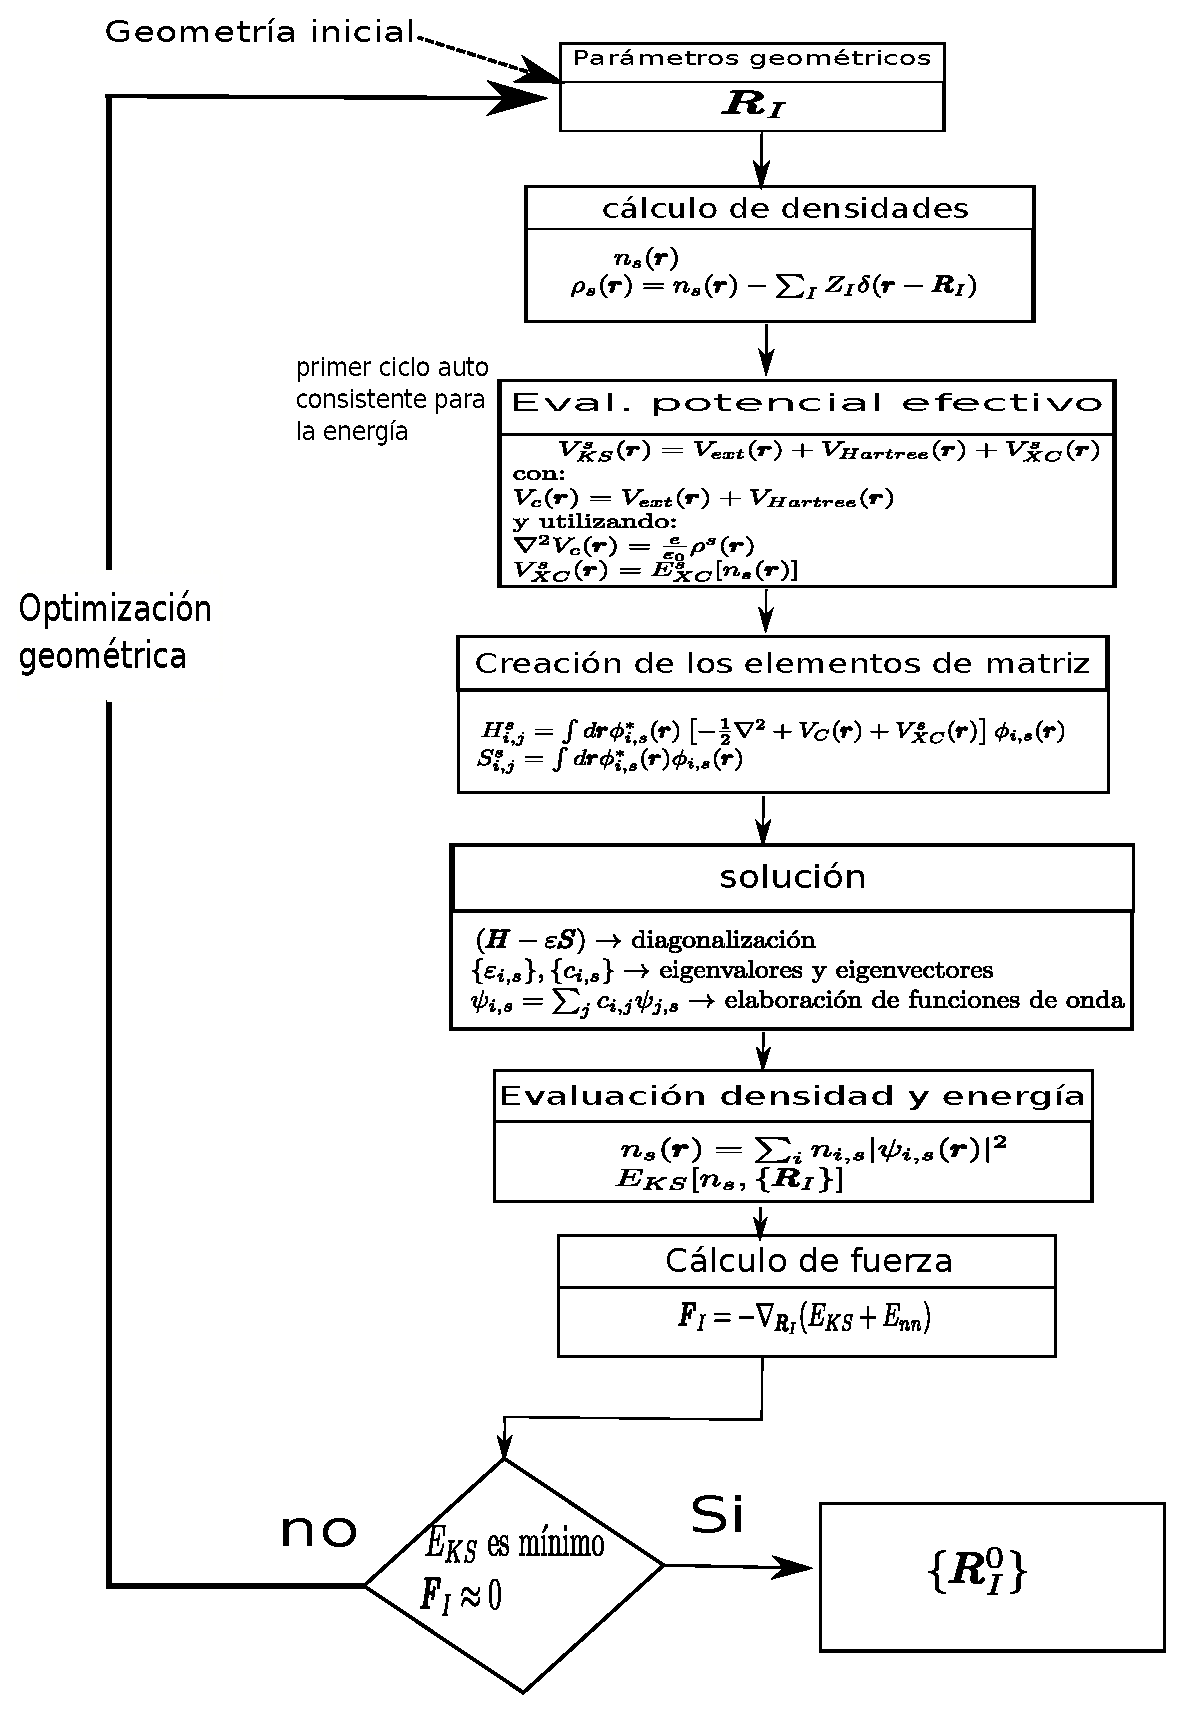
\epsfig{file=figuras/diagramaAuto2.eps, width=8.0cm,height=15.0cm}
   	\caption{ciclo autoconsistente para encontrar la geometr\'ia de equilibrio a partir de una geomietr\'ia inicial $\{\pmb{R}_I^i\} $}
   	\label{fig:esqFuerza}
   \end{figure}
   \newline
   Calculando las fuerzas de Hellman-Feynman utilizando la energ\'ia total (ec. \ref{ec:EnTot2}) se pueden obtener dos componentes
   \begin{equation}
   	\pmb{F}_I = \pmb{F}_I^n + \pmb{F}_I^{el}. \label{ec:FuerzaDesc}
   \end{equation}
   La contribuci\'on debida a la repulsi\'on entre n\'ucleos es
   \begin{equation}
   \pmb{F}_I^n = \sum_{\substack{I,I' = 1 \\ (I \not = I')}}^{N_n} v(\pmb{R}_I - \pmb{R}_{I'}) \frac{\pmb{R}_I - \pmb{R}_{I'}}{|\pmb{R}_I - \pmb{R}_{I'}|^2}
   \end{equation}
   el cual es provocada por la energ\'ia de interacci\'on entre n\'ucleos (ec. \ref{ec:IntII}). Estudiando la contribuci\'on electr\'onica  (ec. \ref{ec:KS_Fuerza})se puede observar que solo el potencial externo $V-{ext} (\pmb{r})$ depende expl\'icitamente de las posiciones nucleares $\{\pmb{R}_I\}$. La densidad $n(\pmb{r})$ depende impl\'icitamente de estas posiciones. Acorde con el teorema de Hellman-Feynman (ec. \ref{ec:HFT}) el gradiente act\'ua sobre el Hamiltoniano. Entonces el \'ultimo t\'ermino en la ecuaci\'on \ref{ec:FuerzaDesc} se puede separar en dos t\'erminos
   \begin{equation}
   \pmb{F}_I^{el} = \pmb{F}_I^{el (1)} + \pmb{F}_I^{el (2)} \label{ec:descFel}
   \end{equation} 
   con
   \begin{equation}
   \pmb{F}_I^{el (1)} = - \int d \pmb{r} ~n(\pmb{r}) \nabla_{\pmb{R}_I} V_{ext} (\pmb{r}) \label{ec:Fel_1}
   \end{equation}
   y
   \begin{equation}
   \pmb{F}_I^{el(2)} = - \int d \pmb{r} \frac{\delta E_{KS} [n]}{\delta n(\pmb{r})} \nabla_{\pmb{R}_I} n(\pmb{r}). \label{ec:Fel_2} 
   \end{equation}
   De acuerdo con el segundo teorema de Hohenberg-Kohn, la ecuaci\'on \ref{ec:Fel_1} se hace cero cuando se logra el estado base del sistema. En tratamientos num\'ericos se pueden considerar fuerzas que se rigen con la ecuaci\'on \ref{ec:Fel_2} las cuales se deben a inexactitudes num\'ericas en e c\'alculo de la dnsidad electr\'onica en el proceso observado en la figura \ref{fig:esqFuerza}. Usando la representaci\'on de la densidad electr\'onica en t\'erminos de los orbitales de kohn-Sham $n(\pmb{r}) = \sum_i n_i |\psi_i (\pmb{r})|^2 $ la fuerza puede ser descrita por
   \begin{equation}
   \pmb{F}_I^{el(2)} = -2 Re \sum_i n_i \int d \pmb{r} [\nabla_{\pmb{R}_I} \psi_i^* (\pmb{r})] \left[-\frac{1}{2} \nabla^2 + V_{KS} (\pmb{r}) - \varepsilon_i \right] \psi_i (\pmb{r}) \label{ec:F2scf}
   \end{equation}
   o
   \begin{eqnarray}
   \pmb{F}_I^{el(2)} = &-& 2 Re \sum_i n_i \int d \pmb{r} [\nabla_{\pmb{R}_I} \psi_i^* (\pmb{r})] \left[-\frac{1}{2} \nabla^2 + \tilde{V}_{KS} (\pmb{r}) -\varepsilon_i \right] \psi_i (\pmb{r}) \nonumber\\ 
   &-& \int d\pmb{r} [V_{KS} (\pmb{r})-\tilde{V}_{KS} (\pmb{r})] \nabla_{\pmb{R}_I} n(\pmb{r}). \label{ec:F2scf_2} 
   \end{eqnarray}
   Con el potencial de Kohn-Sham actuak $\tilde{V}_{KS} (\pmb{r})$ en una cierta iteraci\'on del c\'alculo que genera las funciones de onda $\{\psi_i (\pmb{r})\}$. El primer t\'ermino de la ecuaci\'on \ref{ec:F2scf_2} es cero si los cambios de las funciones de onda mantienen la orto-normalidad cuando un \'atomo se desplaza. Esto sucede con las ondas planas. El segundo t\'ermino mide la no auto consistencia en la soluci\'on de las ecuaciones de Kohn-Sham.
      
   \section{Pseudopotenciales}\label{sec:pseudo}
   \subsection{Introducci\'on a los pseudopotenciales} \label{subsec:introPseudo}
   Es importante puntualizar que el uso de ondas planas solamente da una soluci\'on exacta si el potencial no var\'ia en el espacio, en el caso en que esta variaci\'on sea peque\~na esta se puede tratar como una perturbaci\'on. Es conocido que el potencial generado por los n\'ucleos presenta variaciones considerables en las regiones cercanas a estos, por ejemplo el potencial externo $V_{ext}$ presenta singularidades cerca de las posiciones de los n\'ucleos $\pmb{R_I}$, entonces la expansi\'on de ondas planas de estados electr\'onicos fuertemente ligados y cercanos a los n\'ucleos no es sencillo debido a que se necesitar\'ia una cantidad mucho mayor de ondas planas para poder describir esta regi\'on del potencial, es por esta raz\'on que es conveniente dividir en dos categor\'ias los electrones en el \'atomo: los electrones del n\'ucleo y los electrones de valencia. Los electrones del n\'ucleo son los que ocupan los niveles mas cercanos al n\'ucleo del \'atomo, estos niveles se encuentran completamente ocupados y son electrones muy localizados, debido a su cercan\'ia al n\'ucleo estos no participan en la formaci\'on de enlaces qu\'imicos debido a que se encuentran fuertemente ligados al n\'ucleo; los electrones de valencia son los que determinan la mayor\'ia de las propiedades de los materiales debido a que son los que participan en la formaci\'on del enlace qu\'imico, estos electrones est\'an mas d\'ebilmente ligados al n\'ucleo por lo que es mas f\'acil describirlos con ondas planas porque el potencial que se genera por su interacci\'on con el n\'ucleo es mas suave.  Entonces se sustituye el efecto de los electrones de n\'ucleo con un pseudopotencial de tal forma que se tienen iones y electrones de valencia que interact\'uan entre si, un i\'on est\'a formado por el n\'ucleo y los \'atomos mas fuertemente ligados a estos (electrones de n\'ucleo).
   \newline
   La idea del pseudopotencial se puede explicar distinguiendo entre estados de valencia($v$) y de n\'ucleo ($c$) y utilizando un hamiltoniano de un solo cuerpo $\hat{H} = \hat{T} + \hat{V}$ y escribiendo la ecuaci\'on de Schr\"odinger con $\lambda= c,v$
   \begin{equation*}
   \hat{H} | \psi_{\lambda} \rangle = \varepsilon_{\lambda} | \psi_{\lambda} \rangle 
   \end{equation*}    
   Si se utiliza el m\'etodo OPW (Ortogonalized Plane Wave) se puede construir una pseudo funci\'on de onda $|\tilde{\psi}_v \rangle $ para los electrones de valencia
   \begin{equation*}
   |\tilde{\psi}_v \rangle = | \psi_v \rangle + \sum_c a_{c,v} |\psi_c \rangle
   \end{equation*}
   en la cual se mezcla con los estados de n\'ucleo con $a_{c,v} = \langle \psi_c | \tilde{\psi}_v \rangle \not = 0$ y aun son ortogonales en los estados de n\'ucleo entonces las pseudo funciones de onda satisfacen la ecuaci\'on de  Schr\"odinger
   \begin{equation*}
   \left[\hat{H} + \sum_{c} (\varepsilon_v - \varepsilon_c) |\psi_c \rangle \langle \psi_c |\right] |\tilde{\psi}_v \rangle = \varepsilon_v | \tilde{\psi}_v \rangle
   \end{equation*}
   para los eigenvalores $\{ \varepsilon_v \}$ pero estas funciones $ \{| \tilde{\psi}_v \rangle \}$ son correcciones suavizadas entonces se define el peudo Hamiltoniano $\hat{H}_{ps} = \hat{T} + \hat{V}_{ps}$ con el pseudopotencial
   \begin{equation*}
   V_{ps}= V+ \sum_{c} (\varepsilon_v - \varepsilon_c) |\psi_c \rangle \langle \psi_c |
   \end{equation*}
   el cual es un potencial semilocal en el espacio y dependiente de la energ\'ia.
   \newline
   En el caso de que se tenga un \'atomo aislado en $\pmb{R}_I = 0$ con simetr\'ia esf\'erica $V(\pmb{r}) = V(r)$ y con n\'umeros cu\'anticos $\lambda= n,l,m $, la funci\'on de onda se puede separar en
   \begin{equation}
   \psi_{nlm} (\pmb{r}) = R_{nl} (r) Y_{lm} (\theta, \phi) \label{ec:Psudofunc}
   \end{equation}
   donde $R_{nl}$ representa la parte radial y $Y_{lm} (\theta, \phi) $ son los esf\'ericos arm\'onicos, se puede esperar que el pseudopotencial act\'ue diferente en funciones de distinto momento angular de tal forma que expresan la dependencia de energ\'ia. La forma que tendr\'ia el pseudo potencial es
   \begin{equation}
   V_{ps} = \sum_{l=0}^{\infty} V_{ps}^l (r) \hat{P}_l \label{ec:PseudoV}
   \end{equation} 
   con el pseudopotnecial parcial $V_{ps}^l (r) $ relacionado con el momento angular $l$, y el operador
   \begin{equation}
   \hat{P}_l = \sum_{m=-l}^{l} |lm \rangle \langle lm | \label{ec:psudoProj}
   \end{equation}
   el cual opera en el espacio del $l$-esimo momento angular de tal forma que el pseudopotencial total \ref{ec:PseudoV} es no local.
   \subsection{Peudopotenciales at\'omicos}
   Una propiedad importante en los pseudopotenciales es que puedan se transferibles, es decir que un pseudopotencial que se elabor\'o para cierto sistema se pueda utilizar en otro, en la regi\'on del n\'ucleo tiene que estar "suavizado", es decir que se tiene que limitar la variaci\'on espacial en esta regi\'on. Para construir un pseudopotencial "ab-initio" existen algunas reglas que ayudan a resolver el problema. Se comienza con la ecuaci\'on radial de Shr\"odinger(en unidades de hartree)
   \begin{equation}
   \left\{-\frac{1}{2} \left[\frac{d^2}{dr^2} + \frac{l (l+1)}{2 r^2} \right]+ V(r)\right\} r R_l (\varepsilon,r) = \varepsilon r R_l (\varepsilon,r) \label{ec:ShRadial}
   \end{equation}  
   la cual es una ecuaci\'on de segundo orden y generalmente $\varepsilon$ se fija a $\varepsilon_l$, la soluci\'on se determina por la funci\'on radial $R_l (\varepsilon,r)  $ y su derivada $R'_l (\varepsilon,r)  $  y el potencial$V(r)$ es el potencial de Kohn-Sham (ec. \ref{ec:potKS}) como la suma del potencial de Coulomb de los n\'ucleos, el potencial de Hartree y el de intercambio y correlaci\'on adem\'as de correcciones relativistas (vistas en la secci\'on \ref{sec:corrRel}) 
   \newline
   Las reglas que se tienen que cumplir para construir los pseudopotenciales ab initio son:
   \begin{enumerate}
   	\item Los peudopotenciales reproducen los eigenvalores de energ\'ia $\tilde{\varepsilon}_l$ en acuerdo con aquellos $\varepsilon_l$ obtenidos por un calculo con todos los electrones en los estados de valencia,
   	\begin{equation*}
   	\tilde{\varepsilon}_l = \varepsilon_l.
   	\end{equation*}  
   	\item A una distancia $r$ mayor al radio del n\'ucleo $r_{cl}$ las funciones de la evaluaci\'on exacta son iguales con la evaluaci\'on del pseudopotencial
   	\begin{equation*}
   	\tilde{R}_l (r) = R_l (r)~~~~~~~para~~~~~~r\ge r_{cl}.
   	\end{equation*}
   	\item \label{listNorm}En el caso $r < r_{cl}$ la parte pseudo-radial $\tilde{R}_l (r)$ no tiene nodos y la norma tiene que ser la misma entre el calculo con todos los electrones y la psudo funci\'on de onda, es llamada la condici\'on de la conservaci\'on de la norma
   	\begin{equation*}
   	\int_{0}^{r_{cl}} dr r^2 |\tilde{R}_l (r)|^2 = int_{0}^{r_{cl}} dr r^2 |R_l (r)|^2.
   	\end{equation*}
   	\item Adem\'as una propiedad importante para describir el esparcimiento de las ondas parciales la cual se caracteriza por la fase de esparcimiento $\nu_l (\varepsilon)$ cuya derivada de energ\'ia se relaciona con la derivada logar\'itmica 
   	\begin{equation*}
   	D_l (\varepsilon, r) = \frac{1}{r} \frac{d \ln R_l (\varepsilon, r)}{d \ln r}
   	\end{equation*}
   	y debe de cumplir lo siguiente en $r=r_{cl}$:
   	\begin{equation*}
   	\tilde{D}_l (\varepsilon, r_{cl})= D_l (\varepsilon, r_{cl}) 
   	\end{equation*}
   	
   \end{enumerate}
   En el caso de la \'ultima regla expresa que las propiedades de esparcimiento de dos \'atomos son similares en el rango de energ\'ia $\varepsilon$ de los \'atomos de valencia esto se relaciona con la identidad ($r \le r_{cl} $)
   \begin{equation}
   \frac{d}{d \varepsilon} D_l (\varepsilon, r) = - \frac{2 m }{\hbar} \frac{1}{r^2 R_l ^2 (\varepsilon, r)} \int_{0}^{r} dr' r^{'2} R_l ^2 (\varepsilon, r') \label{ec:freidelSum} 
   \end{equation}
   que corresponde a la regla de suma de Freidel.
   \newline \newline
   El procedimiento para obtener el pseudopotencial  se inicia resolviendo la ecuaci\'on radial de Schr\"odinger para todos los electrones (ec. \ref{ec:ShRadial}) para una configuraci\'on at\'omica y el pesudopotencial puede se elaborado con las reglas mencionadas anteriormente, de acuerdo a la regla \ref{listNorm} el pseudopotencial conserva la norma y existen distintos esquemas para construirlos.
   \newline
   la ecuaci\'on de Schr\"odinger (ec. \ref{ec:ShRadial}) para la pseudo funciones de onda $\tilde{R}_l (r)$ es gobernada para cada momento angular $l$, dado que es influenciado por la interacci\'on de los \'atomos de valencia de densidad $n_v (\pmb{r})$ se puede llamar psudopotencial apantallado, el cual es representado por la siguiente expresi\'on:
   \begin{equation}
   V_{ps}^{(sc)l} (r) = \varepsilon_l + \frac{\hbar}{2m} \left\{-\frac{l (l+1)}{r^2} + \frac{1}{r \tilde{R}_l (r)} \frac{d^2}{dr^2} [r \tilde{R}_l (r)]\right\} \label{ec:PSPot}
   \end{equation}
   donde el n\'umero cu\'antico preincipal $n$ no se muestra para indicar que el c\'alculo est\'a en el nivel base de cada momento angular $l$.Los estados del n\'ucleo entran s\'olo a trav\'es del potencial auto consistente $V(r)$ ,la expresi\'on \ref{ec:PSPot} claramente indica que el pseudopotencial es continuo y la funci\'on $\tilde{R}_l (r)$ se debe desvanecer como $r^l$ para $r \rightarrow 0$ para evitar la singularidad en el origen,adem\'as de que el pseudopotencial depende del estado del momento angular.
   \newline
   El pseudopotencial act\'ua en los estados del momento angular $l$ se obtiene finalmente sustituyendo el efecto de interacci\'on con los electrones de valencia distribuidos acorde a sus pseudo funciones de onda
   \begin{equation}
   v_{ps}^l (r) = V_{ps}^{sc(l)} (r) - \int d^3 r \frac{1}{|\pmb{r}-\pmb{r'}|} \tilde{n}_v^{atomo} (\pmb{r'}) - V_{XC} (\pmb{r}; [\tilde{n}_v^{atomo} (\pmb{r'})]) \label{ec:pseudoSC1}
   \end{equation}   
   con densidad at\'omica esf\'erica:
   \begin{equation}
   \tilde{n}_v^{atomo} (\pmb{r})= \frac{1}{4 \pi} \sum_{l=0}^{l_{max}} \sum_{m=-l}^{l} |\tilde{R}_l (r)|^2. \label{ec:densAtomo}
   \end{equation}
   Si se substrae el efecto de los electrones de valencia se obtiene el pseudopotencial i\'onico (ec. \ref{ec:pseudoSC1}) el cual no depende del ambiente qu\'imico y es transferible.
   \newline
   De acuerdo con la ecuaci\'on \ref{ec:PSPot} cada momento angular $l$ tiene su propio pseudopotencial, de acuerdo con la ecuaci\'on \ref{ec:PseudoV} con el operador de proyecci\'on $\hat{P}_l$ los potenciales parciales se pueden combinar en un pseudopotencial total no local. En el l\'imite $r \rightarrow \infty$ se convierte en un potencial local $- Z^{val} e^2 / (4 \pi \varepsilon_0 r)$ con $Z^{val}$ es el n\'umero de electrones de valencia en el \'atomo, debido a la condici\'on de cerradura del operador de proyecci\'on $\hat{P}_l$ requiere el mismo comportamiento para todo $l$
   \begin{equation*}
   V_{ps}^l (r)= - \frac{Z^{val} e^2}{4 \pi \varepsilon_0 r} ~~~~para ~ r \rightarrow \infty.
   \end{equation*}
   Como consecuencia es \'util descomponer $V_{ps}^l (r)$ en una contribuci\'on de largo alcance e independiente de $l$ y otra dependiente de $l$ y de corto alcance. La de largo alcance es local debido a $\sum_l \hat{P}_l =1$, por esta raz\'on el pseudopotencial es semilocal, son no locales en coordenadas $\theta y \phi$ pero local en la coordenada radial $r$.
   \newline
   Es posible generar un pseudopotencialque incluya la interacci\'on spin-\'orbita . El primer paso es realizar un c\'alculo relativista de todos los electronescon lon n\'umeros cu\'anticos $j=l+\frac{1}{2}$ y $j=l-\frac{1}{2}$ es posible definir un potencial promedio y su diferencia
   \begin{eqnarray*}
   V_{ps}^l (r) &=& \frac{1}{2 l +1} \left[l V_{ps}^{l-\frac{1}{2}} (r) + (l+1) V_{ps}^{l+\frac{1}{2}} (r)  \right] \\
   \Delta V_{ps}^l (r) &=& \frac{1}{2 l +1} \left[V_{ps}^{l+\frac{1}{2}} (r) -  V_{ps}^{l-\frac{1}{2}} (r)  \right]
   \end{eqnarray*} 
   este arreglo da una contribuci\'on adicional a la ecuaci\'on  \ref{ec:PSPot} la cual se puede representar como
   \begin{equation}
   \Delta V_{ps}^{so} = \sum_{l,m} |lm \rangle \Delta V_{ps}^{l} (r)  \pmb{l} \cdot \pmb{s} \langle lm| \label{ec:psudoSO}
   \end{equation}
   con el operador de momento angular $\pmb{l} $ y el operador de spin $\pmb{s}$.
   \subsection{M\'etodo PAW}\label{subsec:PAW}
   E m\'etodo del proyector de ondas aumentadas (PAW, Projector Augmented Wave) es una aproximaci\'on general para la soluci\'on del problema de DFT que reformula el m\'etodo OPW descrito en la secci\'on \ref{subsec:introPseudo}, este m\'etodo introduce proyectores en la soluci\'on del problema de pesudopotencial.
   \newline
   El m\'etodo consiste en tomar una funci\'on "suave" $\tilde{\psi}_i^v (\pmb{r})$ y una transformaci\'on lineal  $\psi^v = \mathcal{T} \tilde{\psi}^v  $ el cual relaciona el conjunto de las funciones de onda $\psi^v $ con la pseudo funciones de onda $ \tilde{\psi}^v$ y se sume que es unitaria excepto por una esfera centrada en el n\'ucleo $\mathcal{T} = \pmb{1}+ \pmb{T}_0$, el los siguiente se omite el exponente v y la etiquetas j para mas simplicidad. En la notaci\'on de Dirac se puede escribir la siguiente ecuaci\'on para la pesudo funci\'on de onda:
   \begin{equation}
   | \tilde{\psi} \rangle = \sum_m c_m | \tilde{\psi}_m \rangle \label{ec:DiracPseudo}
   \end{equation}
   con la funci\'on correspondiente funci\'on de onda,
   \begin{equation}
   |\psi \rangle = \mathcal{T} |\tilde{\psi} \rangle = \sum_m c_m | \psi_m \rangle. \label{ec:DiracAllE}
   \end{equation}
   Entonces la funci\'on de onda en todo el espacio puede es escrita 
   \begin{equation}
   | \psi \rangle = |\tilde{\psi} \rangle + \sum_m c_m \left\{|\psi_m \rangle - |\tilde{\psi}_m \rangle \right\}. \label{ec:DiracFunc}
   \end{equation}
   Si la transformaci\'on $\mathcal{T}$ es lineal, entonces se tiene que cumplir con:
   \begin{equation}
   	c_m = \langle \tilde{p}_m | \tilde{\psi} \rangle   \label{ec:condProj}
   \end{equation}
   para alg\'un proyector $\tilde{p}$ y cumple con la condici\'on de ortogonalidad
   \begin{equation}
   \langle \tilde{p}_m | \tilde{\psi}_{m'} \rangle = \delta_{m,m'} \label{ec:orotoDirac}
   \end{equation}
   entonces la expasi\'on de un centro $\sum_m |\tilde{\psi}_m \rangle \langle \tilde{p}_m | \tilde{\psi} \rangle $ es una func\'ion suave $\tilde{\psi}$ igual a i misma. Para los pseudopotenciales existen muchas opciones para los proyectores y en este m\'etodo la transformaci\'on $\mathcal{T}$ a\'un contiene la funci\'on de onda de todos los electrones
   \begin{equation}
   \mathcal{T} = \pmb{1} + \sum_m \left\{ |\psi_m\rangle - |\tilde{\psi}_m \rangle \right\} \langle \tilde{p}_m |. \label{ec:ProjectorPAW}
   \end{equation}
   Esta expresi\'on aplica tanto para los electrones de valencia como para los electrones de n\'ucleo.
   \newline
   La forma general de las ecuaciones PAW se puede obetener en funci\'on de la transformaci\'on de la ecuaci   contenidos...\'on \ref{ec:ProjectorPAW}, para cualquier operador $\hat{A}$ en el problema considerando todos los electrones, se puede obtener un nuevo operador $\tilde{A}$ que opera en la parte suave de las funciones de onda
   \begin{equation}
   \tilde{A}= \mathcal{T} ^{\dagger} \hat{A} \mathcal{T} = \hat{A} + \sum_{m,m'} |\tilde{p}_m \rangle \left\{\langle \psi_m | \hat{A} | \psi_{m'} \rangle - \langle \tilde{\psi}_m | \hat{A} | \tilde{\psi}_{m'} \rangle \right\} \langle \hat{p}_{m'}| \label{ec:operadorPseudo}
   \end{equation}
   adem\'as se puede sumar a la ecuaci\'on \ref{ec:operadorPseudo} de la forma
   \begin{equation*}
   \hat{B}-\sum_{m,m'} |\tilde{p}_m \rangle \langle \tilde{\psi}_m | \hat{B} | \tilde{\psi}_{m'} \rangle \langle \tilde{p}_{m'}| 
   \end{equation*}
   que no cambia los valores de expectaci\'on. La expresi\'on para la densidad en la teor\'ia PAW se puede expresar como:
   \begin{equation}
   n(\pmb{r}) = \tilde{n} (\pmb{r}) + n^1 (\pmb{r}) - n^1 (\pmb{r}), \label{ec:densidadPAW}
   \end{equation}
   la cual se puede escribir en t\'erminos de los eigenestados $i$ y con las ocupaciones $n_i$ como
   \begin{equation}
   \tilde{n} (\pmb{r}) = \sum_i n_i |\tilde{\psi}_i (\pmb{r})|^2, \label{ec:densPW}
   \end{equation}
   \begin{equation}
   n^1 (\pmb{r}) = \sum_i n_i \sum_{m,m'} \langle \tilde{\psi}_i | \tilde{\psi}_m \rangle \psi_m ^* (\pmb{r}) \psi_{m'} (\pmb{r}) \langle \tilde{\psi}_{m'} | \tilde{\psi}_i \rangle \label{ec:n1} 
   \end{equation}
   y
   \begin{equation}
   \tilde{n}^1 (\pmb{r}) = \sum_i n_i \sum_{m,m'} \langle \tilde{\psi}_i | \tilde{\psi}_m \rangle \tilde{\psi}_m ^* (\pmb{r}) \tilde{\psi}_{m'} (\pmb{r}) \langle \tilde{\psi}_{m'} | \tilde{\psi}_i \rangle. \label{ec:tn1}
   \end{equation}
   Estos dos t\'erminos est\'an localizados en cada \'atomo y las integrales pueden ser coordenadas esf\'ericas. 
   
   \section{correciones relativistas} \label{sec:corrRel}.
   Debido a que el movimiento de los electrones con respecto al n\'ucleo, cuya velocidad es mayor que el movimiento  de n\'ucleo, y debido a la diferencia entre sus masas, es necesario incluir loe efectos relativistas en el movimiento de los electrones, para introducir estos  es necesario utilizar la ecuaci\'on de Dirac:
   \begin{equation}
   i \hbar \frac{\partial \psi}{\partial t} = (c \pmb{\gamma}\cdot \pmb{p} ~+ \gamma_0 m  c^2  ) \psi \label{ec:Dirac}
   \end{equation}
   en donde $\pmb{p } = i \frac{\partial}{\partial \pmb{r}}$ y las matrices $\gamma$ son de dimensi\'on $4 \times 4$ las cuales est\'an dadas para fermiones:
   \begin{equation}
   \gamma_i = 
   \begin{bmatrix}
   0         & \sigma_i \\
   -\sigma_i &    0
   \end{bmatrix},~~i=1,2,3~~y~~
   \gamma_0 =
   \begin{bmatrix}
   \pmb{1}    &   0 \\
      0       &  \pmb{1}
   \end{bmatrix} \label{ec:GammaMatr}
   \end{equation}
    y en donde $\sigma_i$ son las matrices de pauli y $\pmb{1}$ es la matriz unitaria de tama\~no $2 \times 2$.
    \newline
    En donde la soluci\'on tiene la forma
    \begin{equation}
    \psi(x^{\mu}) = e^{-i E t /\hbar} 
    \begin{pmatrix}
    \psi(\pmb{r}) \\
    \chi(\pmb{r})
    \end{pmatrix} \label{ec:solDir}
    \end{equation}
    en donde $x^{\mu} = (\pmb{r},t)$ y $\psi (\pmb{r})$ y $\chi (\pmb{r})$ don las dos componentes del spinor que describen la dependencia espacial y de spin,entonces la ecuaci\'on de Dirac \ref{ec:Dirac} se convierte en ecuaciones acopladas para $\psi$ y  $\chi$:
    \begin{eqnarray}
    c (\sigma \cdot \pmb{p}) \chi &=& (E-m c^2) \psi \nonumber \\
    c (\sigma \cdot \pmb{p}) \psi &=& (E+m c^2) \chi. \label{ec:sistEqDirac}
    \end{eqnarray}
    Las ecuaciones para la interacci\'on de un electr\'on con campos el\'ectrico y magn\'etico se puede derivar remplazando $\pmb{p} \rightarrow \pmb{\pi} = \pmb{p}-(e/c) \pmb{A}$ y $m c^2 \rightarrow mc^2 + e V$ donde $\pmb{A}$ y $V$ son el potencial vectorial y escalar respectivamente los cuales son dependientes del espacio y el tempo. En el caso de materia condensada, al igual que con al ecuaci\'on de Schr\"odinger tambi\'en es necesario hacer una aproximaci\'on utilizando solo los electrones, adem\'as solo se utilizan contribuciones de segundo ordenen la raz\'on de la velocidad del electr\'on y la velocidad de la luz $c$, las cuatro componentes del spinor en la ecuaci\'on de Dirac (ec. \ref{ec:Dirac}) se desacoplan y se obtiene el Hamiltoniano  de Dirac, el Hamiltoniano quasi-relativista de un sistema de electrones en la posici\'on $\pmb{r}_j$ y spin $\pmb{s}_j$ se puede escribir como:
    \begin{multline}
    \hat{H} = \sum_{j=1}^{N} \left\{\frac{1}{2 m_e} [\pmb{p}_j + e \pmb{A} (\pmb{r}_j)]^2 + V_{ext} (\pmb{r}_j)- e V (\pmb{r}_j)\right.\\ \left. {} -\frac{\hbar e}{2 i  (2 m_e c)^2} \pmb{p}_j \cdot [\pmb{E}_{ext} (\pmb{r}_j) + \pmb{E} (\pmb{r}_j)] - \frac{1}{2 m_e (2 m_e c)^2} [\pmb{p}_j + e \pmb{A} (\pmb{r}_j)]^4 \right. \\
    \left. {} + \frac{e}{2 (m_e c)^2} \pmb{s}_j \cdot ([\pmb{E}_{ext} (\pmb{r}_j) + \pmb{E} (\pmb{r}_j)] \times [\pmb{p}_j + e \pmb{A} (\pmb{r}_j)]  ) \right. \\
    \left. {} + \frac{e}{m_e} \pmb{s}_j \cdot \pmb{B} (\pmb{r}_j) \right\} \label{ec:HamilDirac}
    \end{multline}    
    en donde $\pmb{E}_{ext}$ es el campo el\'ectrico inducido por el potencial externo:
    \begin{equation}
    \pmb{E}_{ext} (\pmb{r}) = - \frac{1}{e} \nabla V_{ext} (\pmb{r}) \label{ec:Eext}
    \end{equation}
    con el potencial externo $V_{ext}$ definido por la ecuaci\'on \ref{ec:shVex} de un electr\'on casi-relativista. Adem\'as existe un campo electromagn\'etico cuyas componentes $\pmb{E} (\pmb{r})$ y $\pmb{B} (\pmb{r})$, los cuales est\'an descritos por el potencial escalar $V(\pmb{r})$ y el potencial vectorial $\pmb{A} (\pmb{r})$ de acuerdo con:
    \begin{eqnarray}
    \pmb{E} (\pmb{r}) &=& - \nabla V(\pmb{r}) - \frac{\partial}{\partial t} \pmb{A} (\pmb{r}), \nonumber \\
    \pmb{B} (\pmb{r}) &=& \nabla \times \pmb{A} (\pmb{r}) \label{ec:camposElectromageticos}
    \end{eqnarray}
    los cuales act\'uan en los electrones.
    \newline
    formalmente el Hamiltoniano de la ecuaci\'on \ref{ec:HamilDirac} no contiene la interacci\'on electr\'on-electr\'on de forma explicita, esta interacci\'on se puede introducir  por medio de los campos electromagn\'eticos $\pmb{E} (\pmb{r})$ y $\pmb{B} (\pmb{r})$, los cuales son generados por el movimiento de los electrones en el sistema, para evitar el conteo doble de interacciones de pares, el t\'ermino $-e V (\pmb{r})$ se remplaza por $-\frac{e}{2} V(\pmb{r})$, si $V (\pmb{r})$ est\'a dado por  una interacci\'on de Coulomb entre dos electrones. Otra clase de interacciones tambi\'en est\'an multiplicadas por $\frac{1}{2}$. As\'i mismo las compoalianza morena pesnentes de los campos se representan con operadores en las coordenadas de los electrones.
    \newline
    Los electrones en la posici\'on $\pmb{r}_j$ da lugar al operador de densidad de electrones
    \begin{equation}
    \hat{n} (\pmb{r}) = \sum_{j=1}^{N} \delta (\pmb{r}- \pmb{r}_j) \label{ec:Reln}
    \end{equation}
    y cada electr\'on posee un operador de densidad
    \begin{equation}
    \pmb{v}_j = \frac{i}{\hbar} [\hat{H},\pmb{r}_j]_- \label{ec:Relv}
    \end{equation}
    el cual da lugar a un operador de densidad de corriente
    \begin{equation}
    \hat{\pmb{j}} (\pmb{r}) = \frac{1}{2} \sum_{j=1}^{N} [\pmb{v}_j, \delta (\pmb{r}-\pmb{r}_j)]_+ , \label{ec:Relj}
    \end{equation}
    en donde los corchetes en las ecuaciones \ref{ec:Relv} y \ref{ec:Relj} 
    \begin{equation}
    [\hat{A},\hat{B}]_{\mp} = \hat{A} \hat{B} \mp \hat{B} \hat{A} \label{ec:conm}
    \end{equation} 
    donde $(-)$ denota un conmutador y  $(+)$ un anticonmutador entre los operadores $\hat{A}$ y $\hat{B}$.
    \newline
    El campo electromagn\'etico debido al movimiento de los electrones $\pmb{E} (\pmb{r})$ y $\pmb{B} (\pmb{r})$ se describen con las ecuaciones de Maxwell en el vac\'io con las fuentes $\hat{n} (\pmb{r})$ y $\pmb{\hat{j}} (\pmb{r})$. Estos potenciales (ec. \ref{ec:camposElectromageticos}) cumplen con la condici\'on de invariancia, en este caso se utiliza la invariancia de Coulomb
    \begin{equation}
    \nabla \cdot \pmb{A} (\pmb{r}) = 0. \label{ec:CoulombGauge}
    \end{equation}
    Entonces el potencial escalar se puede obtener con la ecuaci\'on de Poisson
    \begin{equation}
    \nabla^2 V(\pmb{r}) = \frac{e}{\varepsilon_0} \hat{n} (\pmb{r}), \label{ec:poisson}
    \end{equation}
    y entonces el potencial est\'a dado por:
    \begin{equation}
    V(\pmb{r}) = - \frac{e}{4 \pi \varepsilon_0} \int_{\Omega} d \pmb{r'} \frac{\hat{n} (\pmb{r'})}{|\pmb{r}-\pmb{r'}|}= - \frac{1}{e} \sum_{j=1}^{N} v(\pmb{r}-\pmb{r}_j). \label{ec:solPoisson}
    \end{equation}
    \newline
    El potencial vectorial se obtiene de la ecuaci\'on de onda 
    \begin{equation}
    \nabla^2 \pmb{A} (\pmb{r}) - \frac{1}{c^2} \frac{\partial^2 }{\partial t^2} \pmb{A} (\pmb{r}) = \mu_0 e \pmb{\hat{j}} (\pmb{r}) + \frac{1}{c^2} \frac{\partial}{\partial t} \nabla V(\pmb{r}) \label{ec:ecOnda}  
    \end{equation}
    en donde $\mu_0 = 4 \pi \times10^{-7} Vs/Am$ es la permeabilidad del vac\'io.
    \newline
    De acuerdo con la ecuaci\'on \ref{ec:ecOnda} el potencial vectorial $\pmb{A} (\pmb{r})$ est\'a influenciado por los efectos de retardaci\'on y es as\'i mismo un funcional del potencial vectorial dado que el Hamiltoniano (ec. \ref{ec:HamilDirac}) que determina la velocidad de las part\'iculas (ec. \ref{ec:Relv}) aparece en la definici\'on de el operador de la densidad de corriente (ec. \ref{ec:Relj}), es posible tratar este problema de forma autoconsistente expandiendo el Hamiltoniano (\ref{ec:HamilDirac}) hasta las correcciones de segundo orden $~ c^{-2}$ por lo cual se pueden desestimar las primeras correcciones relativistas de la energ\'ia cin\'etica  y lainteracci\'on de spin- \'orbita y entonces se tiene una expresi\'on para la velocidad de la part\'icula
    \begin{equation}
    	\hat{v}_j = \frac{1}{m} \left\{\pmb{p}_j + e \pmb{A} (\pmb{r}_j) + \frac{2i}{\hbar} (\pmb{p}_j \times \pmb{s}_j) \right\} \label{ec:vel_corr}
    \end{equation}  
    en donde los dos primeros t\'erminos se relacionan con el momento electromagn\'etico  del electr\'on y el tercero se relaciona con el movimiento del spin, considerando esto es posible dividir en tres contribuciones al operador de densidad de corriente
    \begin{equation}
    \hat{\pmb{j}} (\pmb{r}) = \hat{\pmb{j}}_p (\pmb{r}) + \hat{\pmb{j}}_d (\pmb{r}) + \hat{\pmb{j}}_s (\pmb{r}) \label{ec:divJ}
    \end{equation}
    en donde
    \begin{equation}
    \hat{\pmb{j}}_p (\pmb{r}) = \frac{1}{2m} \sum_{j=1}^{N} [\pmb{p}_j , \delta(\pmb{r}-\pmb{r}_j)]_+ \label{ec:Jpara} 
    \end{equation} 
    es la densidad de corriente paramagn\'etica,
    \begin{equation}
    \hat{\pmb{j}}_d (\pmb{r}) = \frac{e}{m} \hat{n} (\pmb{r}) \pmb{A} (\pmb{r}) \label{ec:Jdia}
    \end{equation}
    es la densidad de corriente diamagn\'etica y 
    \begin{equation}
    \hat{\pmb{j}}_s (\pmb{r}) (\pmb{r}) = \frac{1}{m} \nabla \times \hat{\pmb{s}}_j (\pmb{r}) \label{ec;Jspin}
    \end{equation}
    es la densidad de corriente de spin, en donde el operador de spin est\'a dado por
    \begin{equation}
    \hat{\pmb{s}} (\pmb{r}) =\frac{\hbar}{2} \sum_{j=1}^{N} \delta (\pmb{r}- \pmb{r}_j) \pmb{\sigma}. \label{ec:SpinOp}
    \end{equation}
    Debido a las restricciones de los t\'erminos $c^{-2}$ la contribuci\'on diamagn\'etica se puede despreciar. Incluyendo los efectos de retardaci\'on, la soluci\'on de la ecuaci\'on \ref{ec:ecOnda} se puede escribir como
    \begin{equation}
    \pmb{A}^{(1)} (\pmb{r}) = - \frac{\mu_0 e}{8 \pi m} \sum_{j=1}^{N} \left\{\frac{\pmb{a}_j}{|\pmb{r}-\pmb{r}_j|} + \frac{[\pmb{a}_j \cdot (\pmb{r}-\pmb{r}_j)] (\pmb{r}- \pmb{r}_j)}{|\pmb{r}-\pmb{r}_j|^3} \right\} \label{ec:SolecOnda}
    \end{equation}
    con el operador generalizado de la velocidad
    \begin{equation}
    \pmb{a}_j = \frac{1}{m} \pmb{p}_j + \frac{2 i }{m \hbar} (\pmb{p}_j \times \pmb{s}_j). \label{ec:genVelocity}
    \end{equation}
    Este operador se introduce en la energ\'ia cin\'etica y el acople entre el spin y el campo magn\'etico en el Hamiltoniano \ref{ec:HamilDirac}. 
    
    \subsection{Componentes relativistas y no relativistas} \label{subsec:rel_norel}
    El Hamiltoniano para electrones cuasi-relativistas (ec. \ref{ec:HamilDirac}) se puede dividir de acuerdo con
    \begin{equation}
    \hat{H} = \hat{H}_0 + \hat{H}_{sr} + \hat{H}_{so} + \hat{H}_{B}. \label{ec:divHamDirac}
    \end{equation} 
    La primera contribuci\'on es el Hamiltoniano  no relativista de los electrones
    \begin{equation}
    \hat{H}_0 = \sum_{j=1}^{N} \left\{\frac{1}{2m} \pmb{p}_j ^2 + V_{ext} (\pmb{r}_j) \right\} + \frac{1}{2} \sum_{\substack{i,j = 1 \\ (i \not = j)}}^{N} v(\pmb{r}_i -\pmb{r}_j) \label{ec:HamnoRel}
    \end{equation} 
    qu contiene la interacci\'on longitudinal  electr\'on-electr\'on utilizando el potencial de coulomb. Las correcciones relativistas escalares son los t\'erminos de Darwin y de correcci\'on de masa
    \begin{equation}
    \hat{H}_{sr} = \frac{1}{2 (2 m c)^2} \sum_{j=1}^{N} \left\{\hbar^2 \nabla^2 [V_{ext} (\pmb{r})-e V(\pmb{r})]_{\pmb{r}= \pmb{r}_j} - \frac{1}{m} \pmb{p}_j ^4 \right\}. \label{ec:HamSR}
    \end{equation}
    El acople spin-\'orbita es 
    \begin{equation}
    \hat{H}_{so} = -\frac{1}{2 (2 m c)^2} \sum_{j=1}^{N} \pmb{s}_j \cdot \left\{\nabla [V_{ext} (\pmb{r})-e V(\pmb{r})]_{\pmb{r}=\pmb{r}_j} \times \pmb{p}_j \right\}. \label{ec:HamSo}
    \end{equation}
    El Hamiltoniano Breit, el cual est\'a relacionado con la interacci\'on transversal de electr\'on-electr\'on, este Hamiltoniano no esta relacionado con la interacci\'on de Coulomb y su expresi\'on es
    \begin{equation}
    \hat{H}_B= \frac{e}{m} \sum_{j=1}^N \left\{\pmb{A}^{(1)} (\pmb{r}_j) \pmb{p}_j + \frac{1}{2} e \left[\pmb{A}^{(1)} (\pmb{r}_j)\right]^2 + \pmb{s}_j \pmb{B}^{(1)} (\pmb{r}_j) \right\}. \label{ec:HamBreit}
    \end{equation}
    El t\'ermino $\left[\pmb{A}^{(1)} (\pmb{r}_j)\right]^2 $ se puede omitir y por lo tanto las contribuciones diamagn\'eticas no se toman en cuenta.
    \newline
    Para un campo magn\'etico casi homog\'eneo se tiene la expresi\'on aproximada
     \begin{equation}
     	\pmb{A}^{(1)} (\pmb{r}) = \frac{1}{2} \pmb{B}^{(1)} (\pmb{r}) \times \pmb{r} \label{ec:Aaprox}
     \end{equation}
    entonces la contribuci\'on de breit (ec. \ref{ec:HamBreit}) toma la forma
    \begin{equation}
    \hat{H}_B = \frac{e}{2m} \sum_{j=1}^N (\pmb{l}_j + 2 \pmb{s}_j) \pmb{B}^{(1)} (\pmb{r}_j) \label{ec:BreitCorr}
    \end{equation}
    donde el operador de momento angular $\pmb{l}= \pmb{r} \times \pmb{p}$ de un electr\'on  individual. Con el operador de momento magn\'etico
    \begin{equation}
    \pmb{m}_j = - \frac{1}{\hbar} \mu_{B} (\pmb{l}_j + 2 \pmb{s}_j) \label{ec:opMagn}
    \end{equation}
    de un electr\'on $j ~~(j=1,...,N)$ y entonces se puede reescribir el Hamiltoniano de Breit (ec. \ref{ec:BreitCorr}) 
    \begin{equation}
    \hat{H}_B = -\sum_{j=1}^N \pmb{m}_j \pmb{B}^{(1)} (\pmb{r}_j) \label{ec:BreitCorr2}
    \end{equation} 
    debido a que $\pmb{m}_j$ y $\pmb{B}^{(1)} (\pmb{r}_j)$ son operadores, la aproximaci\'on \ref{ec:BreitCorr2} permite dar una interpretaci\'on f\'isica de la contribuci\'on de Breit.
    \newline
    En general el potencial vectorial (ec. \ref{ec:SolecOnda}) y el campo magn\'etico resultante (ec. \ref{ec:camposElectromageticos}) se puede dividir en contribuciones orbitales y de spin de acuerdo a la corriente paramagn\'etica y de spin,
    \begin{eqnarray}
    \pmb{A}_{orbita} (\pmb{r}) &=&- \frac{\mu_0 e}{8 \pi m} \sum_{j=1}^N \left\{\frac{\pmb{p}_j}{|\pmb{r}-\pmb{r}_j|} + \frac{[\pmb{p}_j \cdot (\pmb{r}-\pmb{r}_j)](\pmb{r}-\pmb{r}_j)}{|\pmb{r}-\pmb{r}_j|^3} \right\}, \nonumber \\
    \pmb{B}_{orbita} (\pmb{r}) &=& \frac{\mu_0 e}{4 \pi m} \sum_{j=1}^N \frac{(\pmb{r}-\pmb{r}_j)}{|\pmb{r}-\pmb{r}_j|^3}, \nonumber \\
    \pmb{A}_{spin} (\pmb{r}) &=& \frac{\mu_0 e}{4 \pi m} \sum_{j=1}^N \frac{(\pmb{r}-\pmb{r}_j)}{|\pmb{r}-\pmb{r}_j|^3} \times \pmb{s}_j, \\
    \pmb{B}_{spin} (\pmb{r}) &=&- \frac{\mu_0 e}{4 \pi m} \sum_{j=1}^N \left\{\frac{\pmb{s}_j}{|\pmb{r}-\pmb{r}_j|^3} -3 \frac{[\pmb{s}_j \cdot (\pmb{r}-\pmb{r}_j)](\pmb{r}-\pmb{r}_j)}{|\pmb{r}-\pmb{r}_j|^5} \right\}. \nonumber 
    \end{eqnarray} 
    Estos campos permiten re escribir la expresi\'on \ref{ec:HamBreit}   
    \begin{equation}
    \hat{H}_B= \frac{e}{2m} \sum_{j=1}^N \left\{\pmb{A}_{orbita} (\pmb{r}_j) \cdot \pmb{p}_j + \pmb{A}_{spin} (\pmb{r}_j) \cdot \pmb{p}_j + \pmb{B}_{orbita} (\pmb{r}_j) \cdot \pmb{s}_j +\pmb{B}_{spin} (\pmb{r}_j) \cdot \pmb{s}_j \right\} \label{ec:breitHam}
    \end{equation}
    donde se introduce el factor $\frac{1}{2}$ para considerar el doble conteo de interacciones pares en sistemas magn\'eticos o con polarizaci\'on de spines. El primer t\'ermino es una correcci\'on de la interacci\'on entre dipolos magn\'eticos de los electrones, los cuales resultan del movimiento orbital de los electrones. El segundo y tercer t\'ermino est\'an relacionados con las interacciones spin-\'orbita y \'orbita-spin en adici\'on de la interacci\'on spin -\'orbita expresada en la ecuaci\'on \ref{ec:HamSo} que se relaciona con los campos el\'ectricos internos. Estos describen el acople entre momentos magn\'eticos orbitales y momentos magn\'eticos de spin. El \'ultimo t\'ermino representa la interacci\'on spin-spin entre momentos magn\'eticos y el cual tiene la forma de la interacci\'on dipolo-dipolo magn\'etico. El Hamiltoniano de Breit se puede re escribir como
    \begin{multline}
    \hat{H}_B = \frac{e^2}{4 \pi \varepsilon_0} \frac{1}{(2 m c)^2} \sum_{\substack{i,j = 1 \\ (i \not = j)}} \left\{- \frac{1}{|\pmb{r}_i-\pmb{r}_j|} \left[\pmb{p}_i \cdot \pmb{p}_j + \frac{[\pmb{p}_i \cdot (\pmb{r}_i-\pmb{r}_j)][\pmb{p}_j \cdot (\pmb{r}_i-\pmb{r}_j)]}{|\pmb{r}_i-\pmb{r}_j|^2} \right] \right. \\ \left. {} + \frac{4}{|\pmb{r}_i-\pmb{r}_j|^2} \pmb{s}_j \cdot \left(\frac{\pmb{r}_i-\pmb{r}_j}{|\pmb{r}_i-\pmb{r}_j|} \times \pmb{p}_j \right) \right. \\
    \left. {} + \frac{2}{|\pmb{r}_i-\pmb{r}_j|^3} \left[\pmb{s}_i \cdot \pmb{s}_j - 3 \frac{[\pmb{s}_i \cdot (\pmb{r}_i - \pmb{r}_j)][\pmb{s}_j \cdot (\pmb{r}_i - \pmb{r}_j)] }{|\pmb{r}_i-\pmb{r}_j|^2} \right] \right\}. \label{ec:HamBreit2}
    \end{multline}
    La auto interacci\'on del electr\'on no se considera y las interacciones son cuadr\'aticas en la raz\'on de la velocidad del electr\'on y la velocidad de la luz.
    \subsection{tratamiento de las correcciones relativistas } \label{subsec:tratamientoRel}
    La parte mas importante del Hamiltoniano para la interacci\'on entre electrones en un campo $V_{ext} (\pmb{r})$ de los n\'ucleos est\'a dada principalmente por la parte no relativista de la ecuaci\'on \ref{ec:HamilDirac}, es la contribuci\'on  $\hat{H}_0$ dada por la ecuaci\'on \ref{ec:HamnoRel}, la cual contiene la interacci\'on  longitudinal entre electrones. En muchos c\'odigos utilizados para realizar c\'alculos de primeros principios (incluido Quantum-Espresso) incluyen las correcciones relativistas escalares $\hat{H}_{sr}$ (ec. \ref{ec:HamSR} ) a las energ\'ias cin\'etica y potencial en la construcci\'on de los pseudopotenciales. Debido a que las correcciones relativistas escalares son muy peque\~nas $\hat{H}_{sr}\sim c^{-2}$ as\'i como la interacci\'on de spin-\'orbita $\hat{H}_{so}$, por lo cual es necesario realizar una nueva aproximaci\'on partiendo del remplazo operador de campo el\'ectrico $\pmb{E} (\pmb{r}) $ por su valor de expectaci\'on $ \langle \pmb{E} (\pmb{r}) \rangle = \langle \Psi | \pmb{E} (\pmb{r}) | \Psi \rangle $. las fluctuaciones $\Delta \pmb{E} (\pmb{r}) = \pmb{E} (\pmb{r}) - \langle \pmb{E} (\pmb{r}) \rangle $ no est\'an siendo consideradas, por lo tanto el potencia de interacci\'on entre los electrones $-e V (\pmb{r})$ es sustituido por su valor de expectaci\'on $ \langle V (\pmb{r}) \rangle = \langle \Psi | V (\pmb{r}) | \Psi \rangle $, entonces las correcciones relativistas $V_{ext} (\pmb{r}) - e V(\pmb{r})$ son remplazadas por un potencial efectivo  $V_{eff}^{sr} (\pmb{r})$, entonces $V_{eff}^{sr} (\pmb{r}) \approx V_{ext} (\pmb{r}) -e V (\pmb{r}) $ es calculado utilizando una aproximaci\'on al potencial de Hartree y la contribuci\'on de intercambio y correlaci\'on. En lugar de la ecuaci\'on  \ref{ec:HamSR} se tiene la siguiente expresi\'on:
    \begin{equation}
    \hat{H}_{sr} = \frac{1}{2 (2mc)^2} \sum_{j=1}^N \left\{\hbar^2 \nabla^2  V_{eff}^{sr} (\pmb{r}) |_{\pmb{r}= \pmb{r}_j} - \frac{1}{m} \pmb{p}_j^4\right\}. \label{ec:HamSR_Mean}
    \end{equation}
    Y en el caso de la interacci\'on spin-\'orbita
    \begin{equation}
    \hat{H}_{so} =- \frac{1}{2 (mc)^2} \sum_{j=1}^N \pmb{s}_j \cdot \left\{ \nabla  V_{eff}^{sr} (\pmb{r}) |_{\pmb{r}= \pmb{r}_j} \times \pmb{p}_j\right\}. \label{ec:HamSO_mean}
    \end{equation}
    El gradiente de $V_{eff}^{sr} (\pmb{r})$ indica los efectos relativistas del movimiento del electr\'on cerca del n\'ucleo, en  orden de tratarlos se puede observar que el potencial puede ser dividido en contribuciones de esas regiones. De acuerdo con la ecuaci\'on \ref{ec:shVex}  se puede descomponer como
    \begin{equation}
    V_{eff}^{sr} (\pmb{r}) = \sum_{I=1}^{N_n} \tilde{V}_{eff}^{sr} (|\pmb{r}- \pmb{R}_I|) \label{ec:descVeffSR}
    \end{equation}  
    con las contribuciones $\tilde{V}_{eff}^{sr} (|\pmb{r}|)$ se asumen que tienen simetr\'ia esf\'erica cerca de la posici\'on del n\'ucleo $\pmb{R}_I$. Con $\nabla  \tilde{V}_{eff}^{sr} (r) = \frac{1}{r} \left[\frac{d}{dr} \tilde{V}_{eff}^{sr} (r) \right]$ y con la abreviaci\'on $r = |\pmb{r}|$ el Hamiltoniano de spin-\'orbita (ec. \ref{ec:HamSO_mean}) se puede escribir como
    \begin{equation}
    \hat{H}_{so} =- \frac{1}{2 (mc)^2} \sum_{I=1}^{N_n} \sum_{j=1}^N \frac{1}{r} \frac{d}{dr} \tilde{V}_{eff}^{sr} (r) |_{r=|\pmb{r}_j -\pmb{R}_I|} \pmb{s}_j \cdot \pmb{l}_{j,I}  \label{ec:HamSO_mean_esf}
    \end{equation}
    con el operador de momento angular $\pmb{l}_{j,I} = (\pmb{r}_j - \pmb{R}_I) \times \pmb{p}_j$ de un electr\'on $j$ y un n\'ucleo $I$. Esta representaci\'on de la interacci\'on spin-\'orbita sugiere una unificaci\'on con la energ\'ia potencial de los electrones debido a su interacci\'on con los n\'ucleos porque en t\'erminos de la ecuaci\'on \ref{ec:HamSO_mean_esf} el potencial externo  $V_{ext} (\pmb{r}) $ (ec. \ref{ec:shVex}) se puede generalizar a un potencial dependiente del spin $\tilde{V}_{ext} (\pmb{r}, \pmb{s})$ el cual proviene de la suma sobre las posiciones de los n\'ucleos. El uso de este potencial tiene como principal problema el requerimiento de utilizar un tratamiento no colineal para $\pmb{s}$ y se requiere una evaluaci\'on auto consistente para $V(\pmb{r})$. Para la implementaci\'on en un c\'odigo se utiliza una aproximaci\'on local del factor $\frac{1}{r} \tilde{V}_{eff}^{sr} (r) $. Utilizando el hecho de que s\'olo la regi\'on cercana al n\'ucleo contribuye se restringe el c\'alculo de  la interacci\'on spin-\'orbita a una regi\'on dentro de una esfera alrededor del n\'ucleo.
    \newline
    Para la interacci\'on de Breit, debido a que es muy peque\~na, tambi\'en se utiliza una aproximaci\'on de campo medio. Partiendo de la expresi\'on  \ref{ec:BreitCorr2} que describe esta energ\'ia en funci\'on del momento magn\'etico $\pmb{m}_j$ (ec. \ref{ec:opMagn}) de los electrones, estos dipolos magn\'eticos generan un campo magn\'etico $\pmb{B}^{(1)} (\pmb{x}) $ de acuerdo con la expresi\'on
    \begin{equation}
    \pmb{B}^{(1)} (\pmb{r}) = - \frac{\mu_0}{4 \pi } \sum_{j=1}^N \left[ \frac{\pmb{m}_j}{|\pmb{r}-\pmb{r}_j|^3} - 3 \frac{[\pmb{m}_j \cdot (\pmb{r}-\pmb{r}_j)](\pmb{r}-\pmb{r}_j)}{|\pmb{r}-\pmb{r}_j|^5} \right]. \label{ec:B1}
    \end{equation} 
    introduciendo esta ecuaci\'on en la expresi\'on \ref{ec:BreitCorr2} con un factor de $\frac{1}{2}$ para evitar el doble conteo de interacciones, se puede encontrar la siguiente expresi\'on para la interacci\'on de Breit
    \begin{equation}
    \hat{H}_B = - \frac{\mu_0}{8 \pi } \sum_{\substack{i,j = 1 \\ (i \not = j)}}^N \left[ \frac{\pmb{m}_i \cdot \pmb{m}_j}{|\pmb{r}-\pmb{r}_j|^3} - 3 \frac{[\pmb{m}_i \cdot (\pmb{r}_i-\pmb{r}_j)][\pmb{m}_j \cdot (\pmb{r}-\pmb{r}_j)]}{|\pmb{r}_i-\pmb{r}_j|^5} \right]. \label{ec:BreitCorr3}
    \end{equation}
    el cual corresponde a una interacci\'on cl\'asica de dipolos magn\'eticos. Una aproximaci\'on de campo medio es remplazar el operador del dipolo $\pmb{m}_j$ por su valor de expectaci\'on $\langle \pmb{m}_j \rangle$, entonces el valor de expectaci\'on de l Hamiltoniano de Breit $\hat{H}_B$ describe una energ\'ia de interacci\'on cl\'asica. 
     
    \chapter{Materiales Bidimensionales}
    
    

\end{document} 